\chapter{Le Grand Collisionneur de Hadrons (LHC)}
\renewcommand\chapterillustration{LHC/lhc}
\ThisULCornerWallPaper{1}{\chapterillustration}
\minitoc
\lettrine[lines=4, slope=-0.5em]{C}{e} chapitre décrit le complexe des accélérateurs de particules du CERN\footnote{Organisation Européenne pour le Recherche Nucléaire (laboratoire européen de physique des particules).}. Le but étant d'obtenir un faisceau de particules avec une énergie suffisante pour être injecté dans le Grand Collisionneur de Hadrons (LHC\footnote{Large Hadron Collider.}) et ainsi atteindre une énergie finale de \SI{7}{\tera\eV}. De nombreux résultats obtenus durant cette thèse ont nécessité l'utilisation d'accélérateurs de ce complexe. Une description du LHC est également donnée, car ses performances présentes et futures déterminent les choix technologiques des détecteurs utilisant son faisceau.

\section{Le complexe d'accélérateurs du CERN}

Le complexe d'accélération (cf.Fig~\ref{complexe}) du CERN est une série de machines qui délivrent des faisceaux de particules d'énergies de plus en plus élevées. Chaque machine accélère les faisceaux et les injecte dans la machine suivante. Le dernier accélérateur du complexe est le LHC.

Le programme de ce dernier est surtout basé sur des collisions proton-proton. Cependant chaque année, environ un mois est consacré aux collisions d'ions lourds (plomb-plomb) ou (proton-plomb) afin d'étudier notamment le plasma de quarks et gluons, l'une des phases de l'Univers peu après le Big Bang. Dans le cas de ces collisions, la chaine d'accélération est constituée du \textit{Linear Accelerator} \num{3} (LINAC \num{3}) et du \textit{Low Energy Ion Ring} (LEIR) utilisé pour le stockage des ions et leur refroidissement. La chaine d'accélération est ensuite identique à celle pour les collisions proton-proton.

\vspace{1cm}
\begin{minipagewithmarginpars}[ht!]{0.95\textwidth}
	\vspace*{0.5cm}
  	\centering
	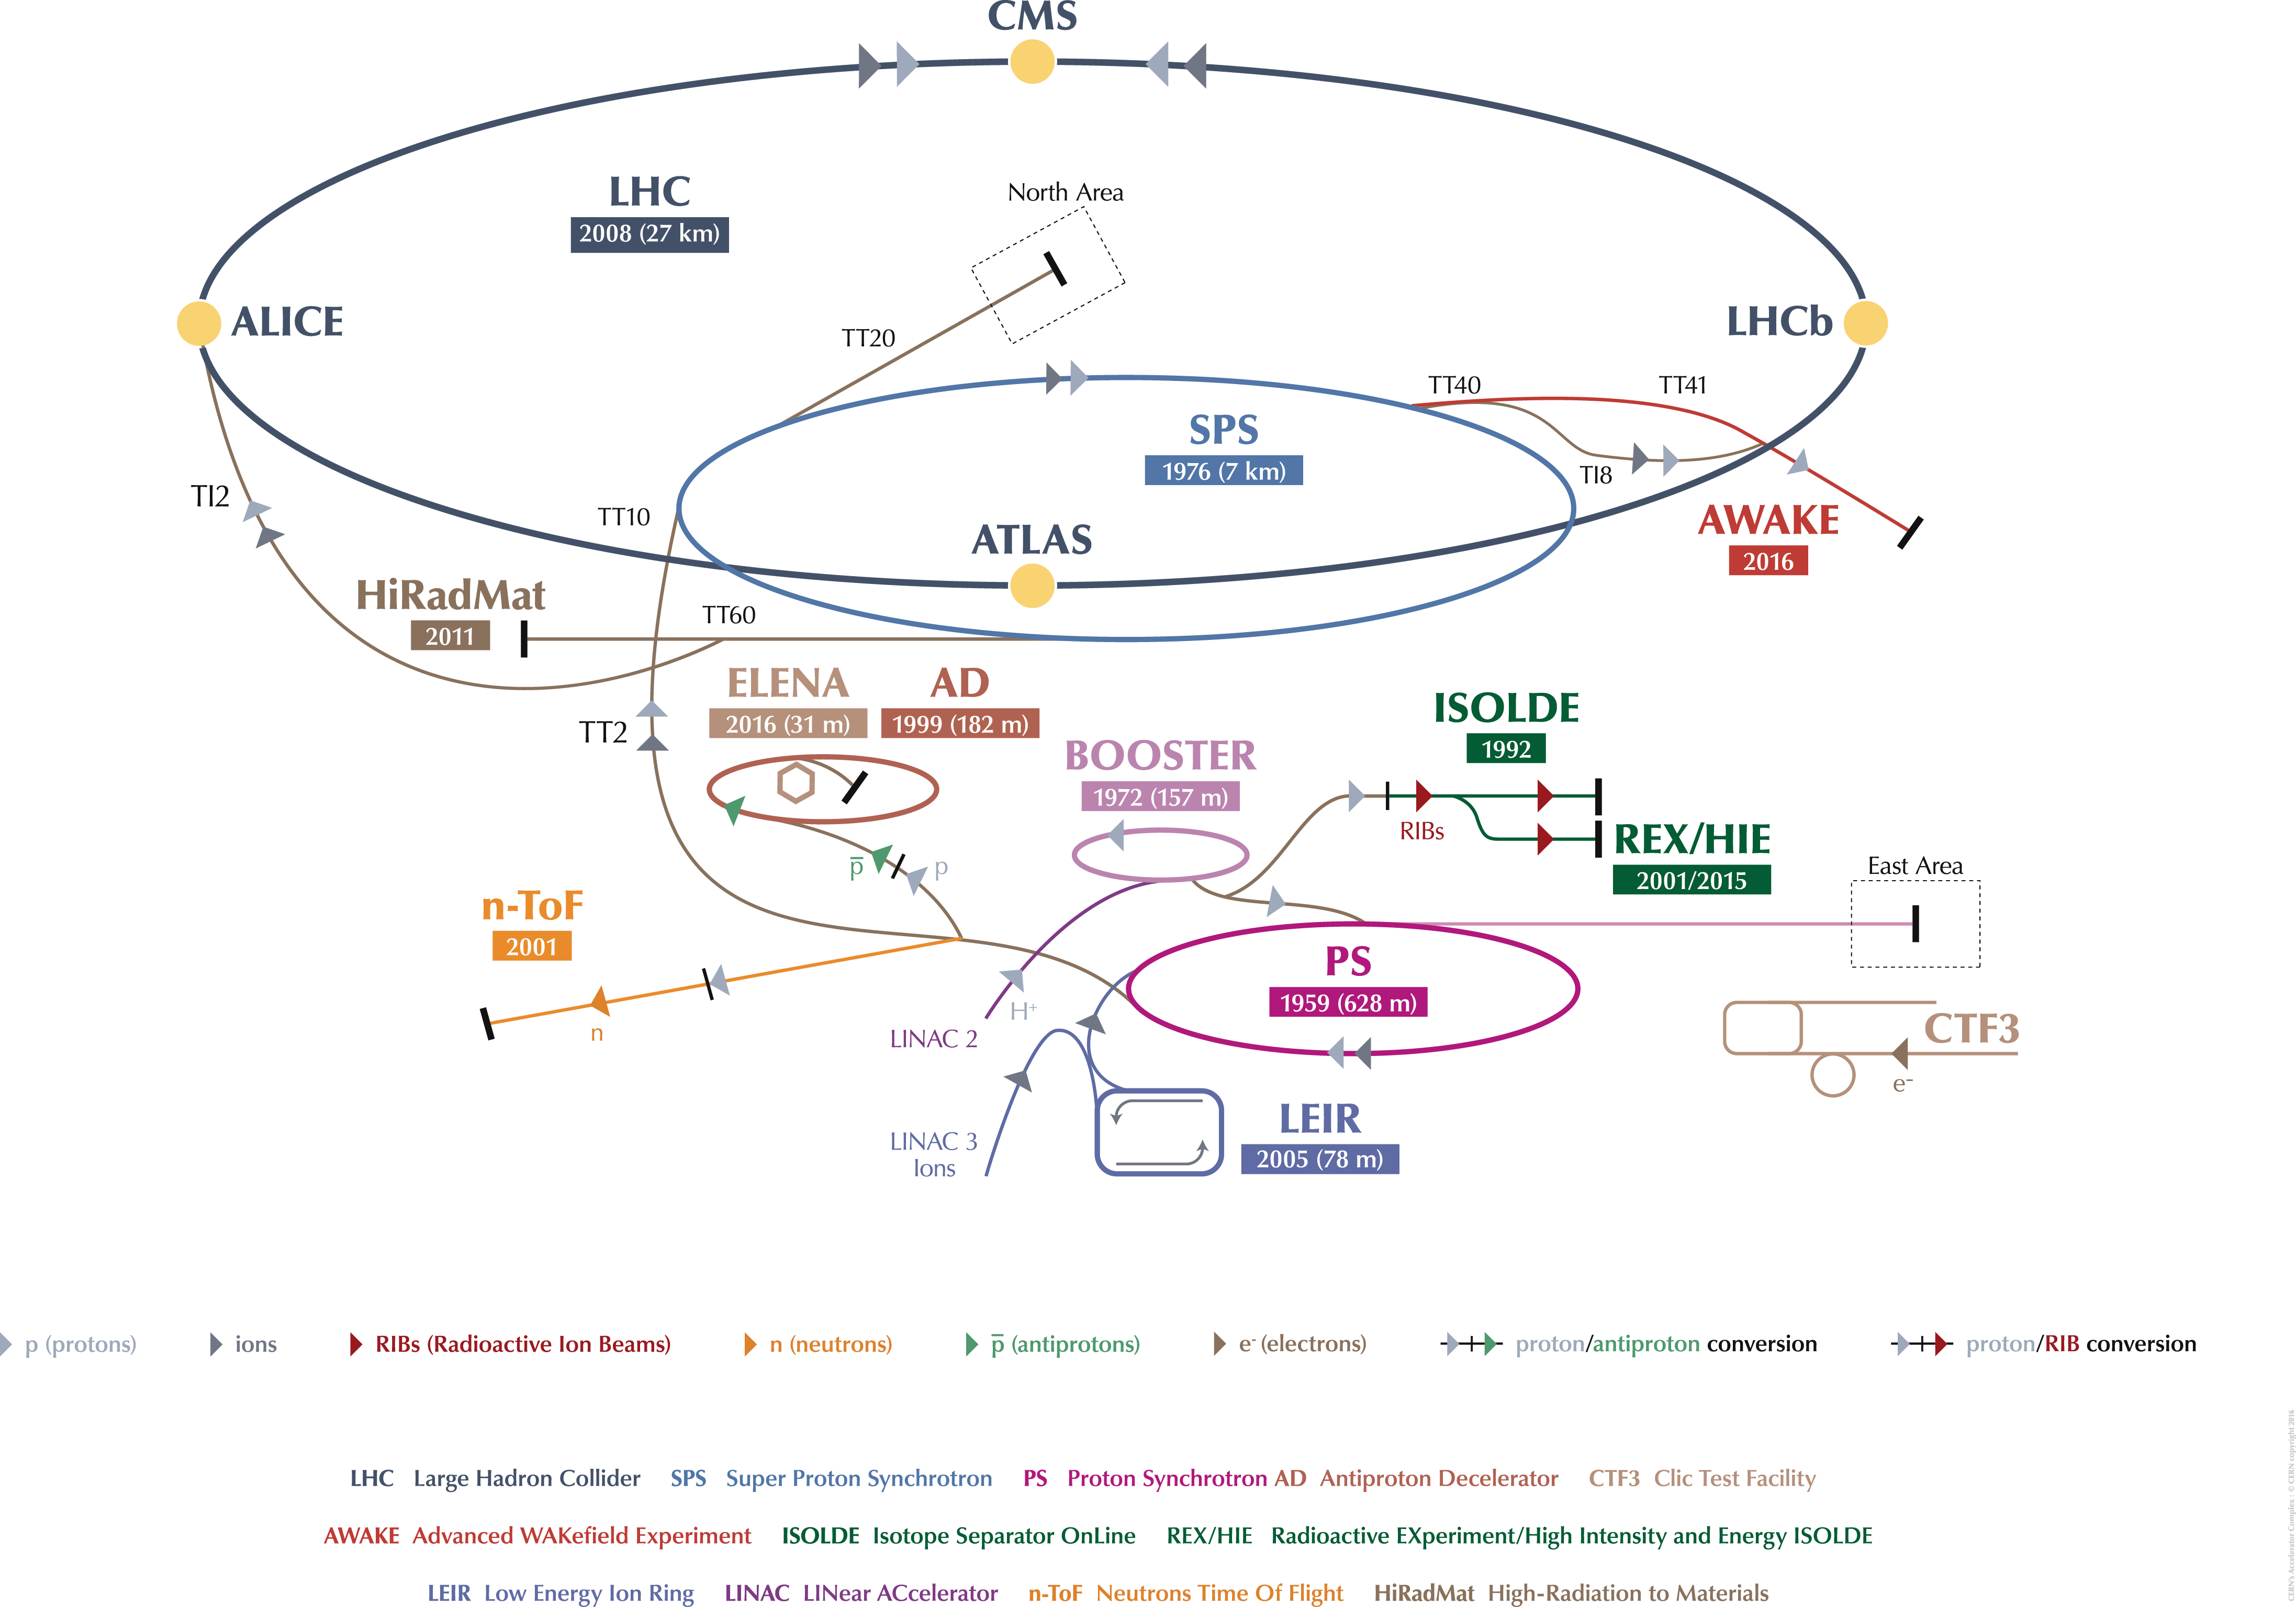
\includegraphics[scale=0.40]{LHC/complexe.png}
  	\captionof{figure}{Schéma du complexe d'accélération du CERN. La chaine d'injection du LHC est constituée du Linac \num{2}, du Booster, du PS et du SPS.}
  	\label{complexe}
  	\par 		
\end{minipagewithmarginpars}

\marginpar
{
	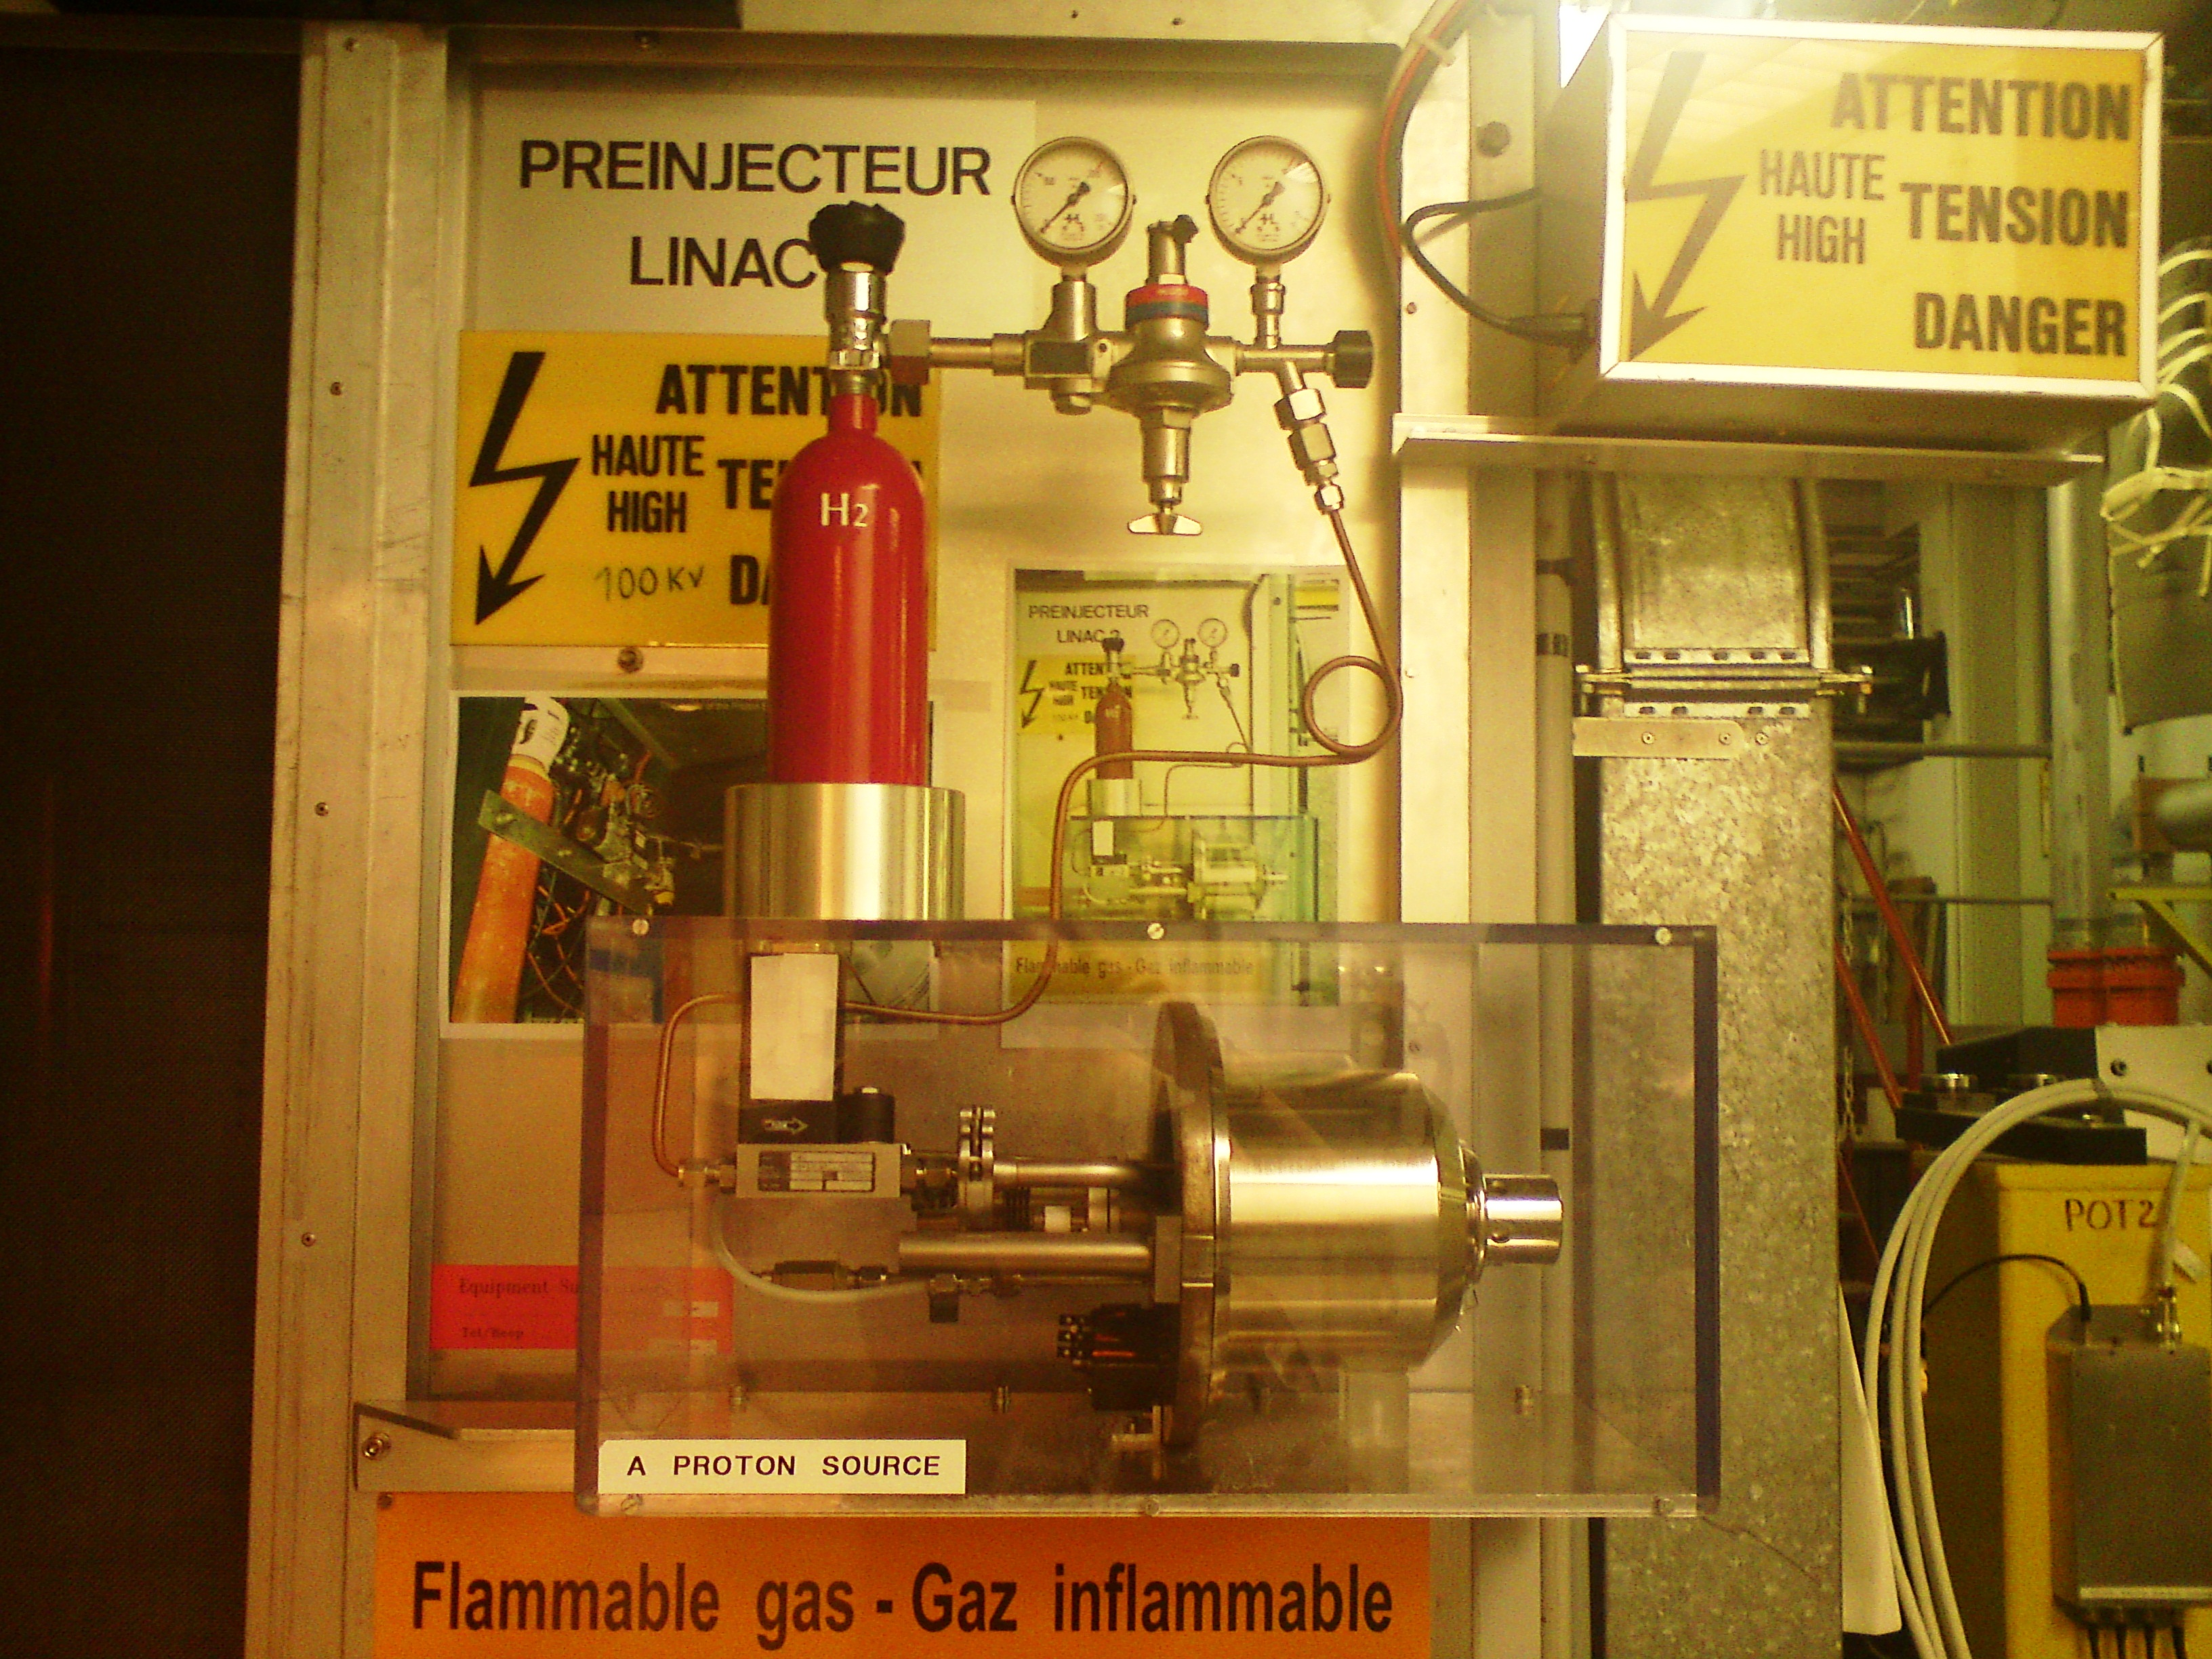
\includegraphics[width=\marginparwidth]{LHC/Bouteille.jpg}
	\captionof{figure}{Source de protons du LHC.}
	\label{bouteille}	
}
\marginpar
{
	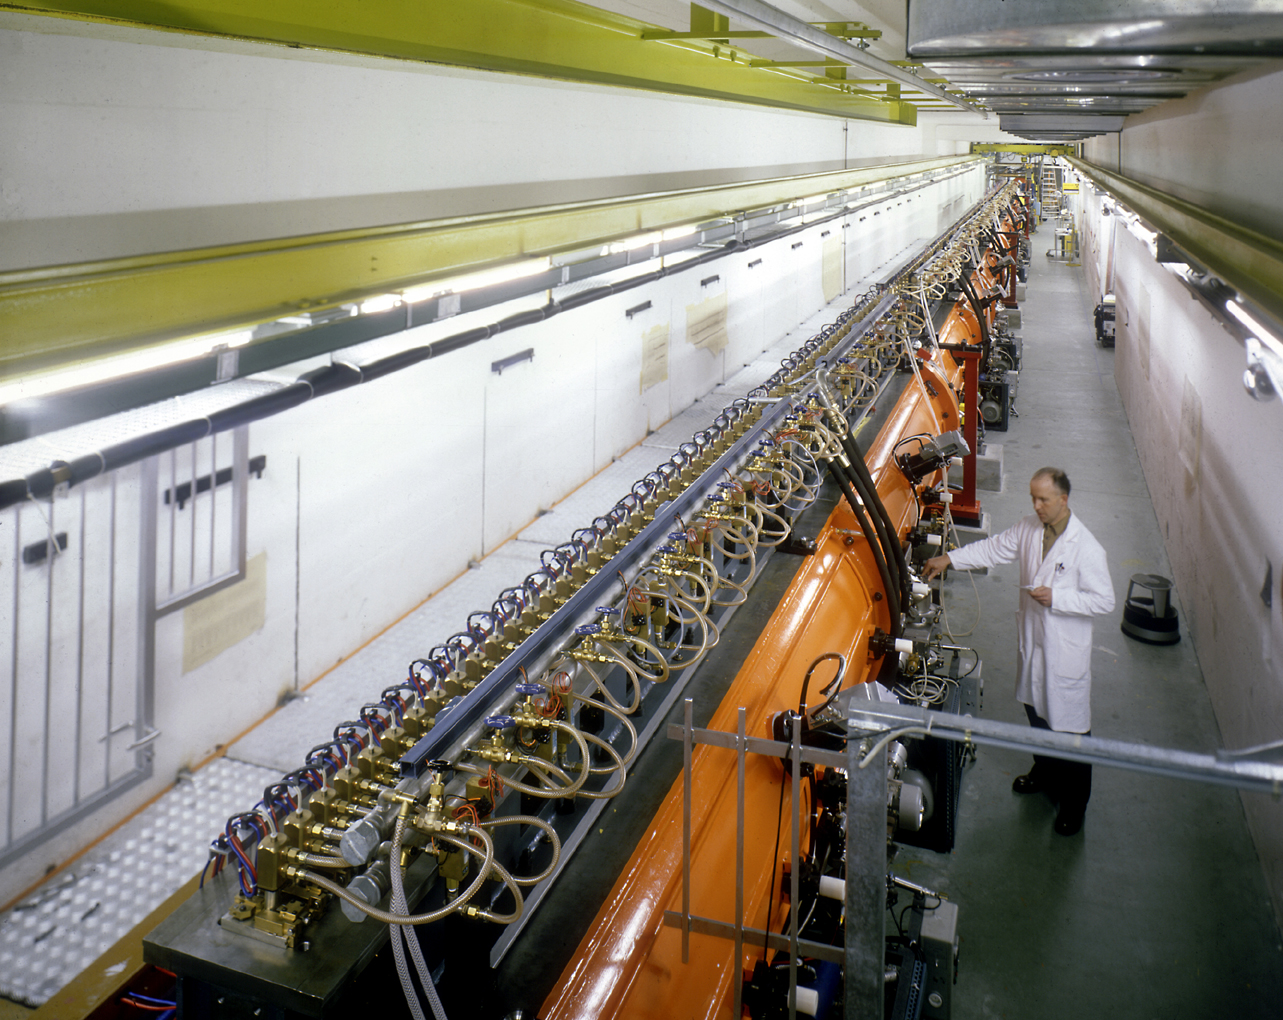
\includegraphics[width=\marginparwidth]{LHC/linac2.jpg}
    \captionof{figure}{Photo du LINAC \num{2}.}
    	\label{linac2}
}

\marginpar
{
	
	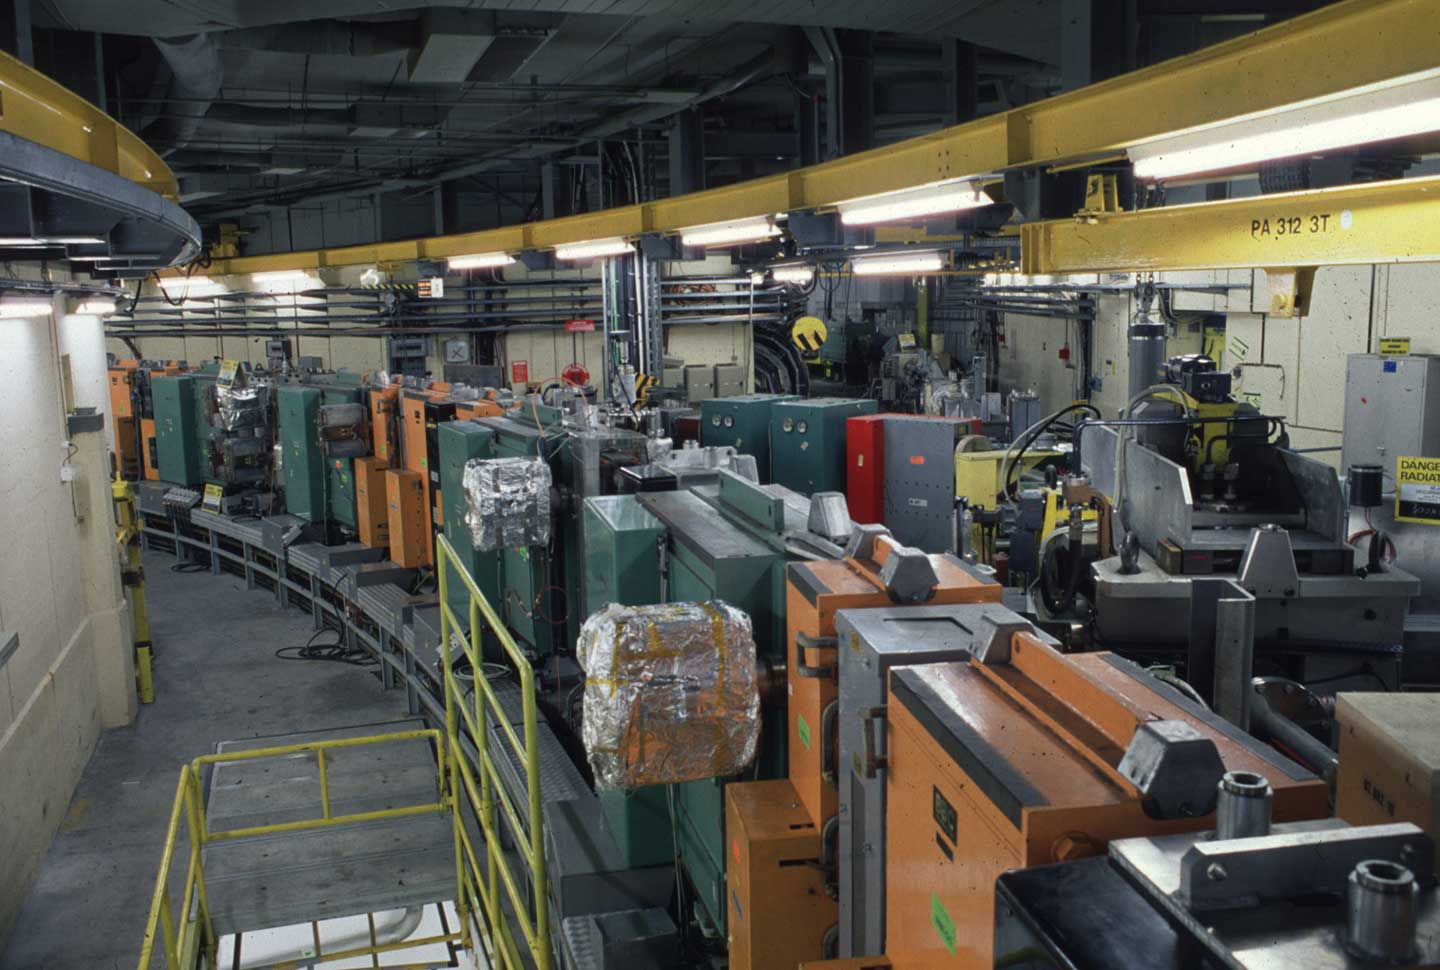
\includegraphics[width=\marginparwidth]{LHC/booster.jpg}
    \captionof{figure}{Photo du Booster du Synchrotron à protons.}
    	\label{booster}
}

\marginpar
{
	
	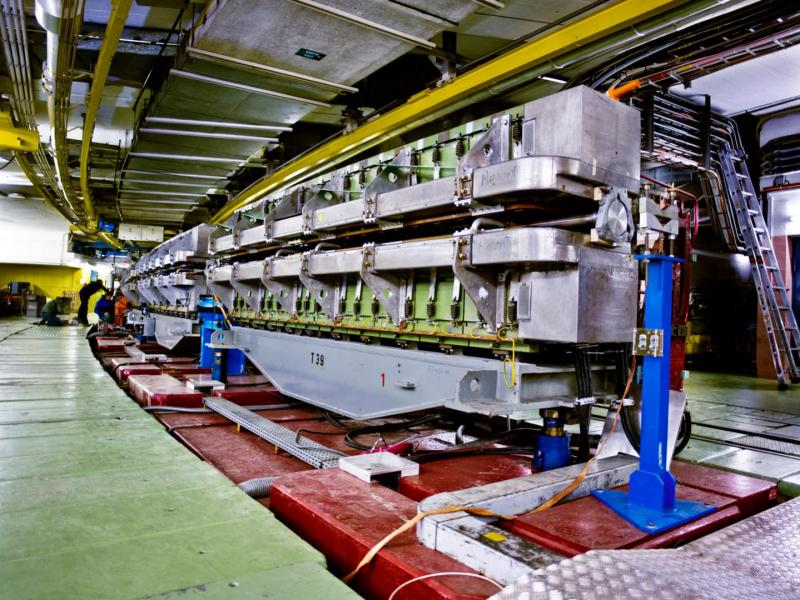
\includegraphics[width=\marginparwidth]{LHC/ps.jpg}
    \captionof{figure}{Photo du PS.}
    	\label{ps}
}

\marginpar
{
	
	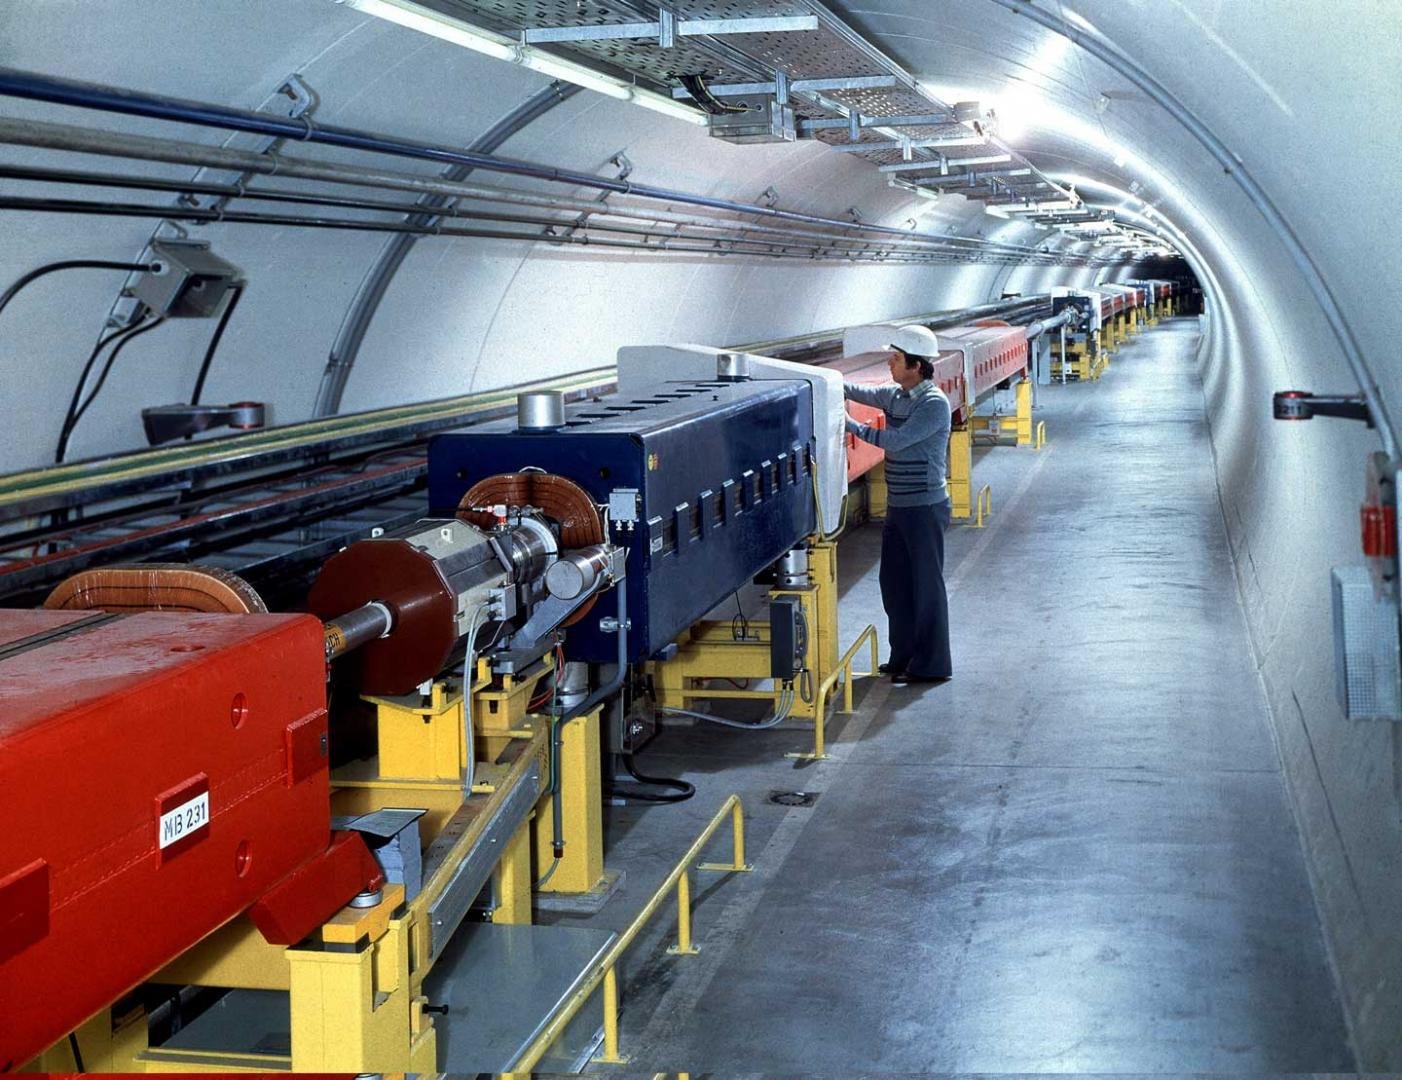
\includegraphics[width=\marginparwidth]{LHC/sps.jpg}
    \captionof{figure}{Photo du SPS.}
    	\label{sps}
}
Pour les collisions proton-proton, la source de protons est une bouteille de dihydrogène gazeux (cf.Fig~\ref{bouteille}). Les atomes d’hydrogène sont injectés dans le \textit{Duoplasmatron Proton IOn Source}, où il sont chauffés et soumis à un champ électrique qui arrache leur électron et les ionise en $H^{+}$ (proton). Les protons extraits sont ensuite envoyés dans l'accélérateur linaire (LINAC 2 (cf.Fig~\ref{linac2})) où ils atteignent l'énergie de \SI{50}{\mega\eV}. Leur vitesse est alors d'environ \SI{0.3}{\c} où $c$ est la vitesse de la lumière dans le vide ($c=$\SI{299 792 458}{\meter\per\second}). Ils parcourent ensuite les \num{4} anneaux de \SI{157}{\meter} de circonférence du Booster du Synchrotron à protons (BOOSTER (cf.Fig~\ref{booster})) qui les amènent à une énergie de \SI{1.4}{\giga\eV} avant de les injecter dans l'accélérateur suivant, le Synchrotron à protons (PS (cf.Fig~\ref{ps})). Cet accélérateur circulaire de \SI{628}{\meter} de circonférence, permet aux faisceaux d'atteindre une énergie de \SI{25}{\giga\eV} et une vitesse de \SI{0.87}{\c}. Il sert aussi à préparer le faisceau en le découpant en série de paquets (\textit{bunchs}) de particules nécessaires au LHC. Ces \textit{bunchs} sont ensuite envoyés dans le supersynchrotron à protons (SPS (cf.Fig~\ref{sps})) d'une circonférence de \SI{7}{\kilo\meter}, où l'énergie du faisceau atteint \SI{450}{\giga\eV} soit une vitesse de \SI{0.99}{\c}. Les paquets sont regroupés pour former des trains de paquets avant d'être enfin envoyés dans le Grand Collisionneur de Hadrons (LHC). L'injection et le guidage de faisceaux d'une telle énergie par des aimants supraconducteurs rapides est une tâche délicate, la moindre erreur pourrait détériorer l'accélérateur. Afin de vérifier les paramètres, un faisceau de test de faible intensité \textit{"pilot beam"} est donc injecté. Ensuite, le faisceau de haute énergie, séparé en deux, est injecté dans deux conduits différents, l'un circulant dans un sens et l'autre dans le sens contraire. Ces faisceaux sont ensuite accélérés jusqu'à une énergie de $\sim$\SI{7}{\tera\eV} et ne se croisent qu'aux points d'interactions. À ce stade, les protons ont une vitesse de \SI{0.999999991}{\c}, soit \SI{299 792 455,3}{\meter\per\second}. Ils ne se déplacent que \SI{2.7}{\meter\per\second} moins vite que la lumière. Afin d'accélérer les protons à une vitesse si proche de celle la lumière, d'importantes contraintes de pression et de température sont nécessaires. Un vide poussé est impératif à l'intérieur du LHC afin de minimiser les interactions, la pression interne est de l'ordre de \SI{e-13}{\atm} soit \num{10} fois moins que la pression à la surface de la Lune. La présence d'aimants supraconducteurs nécessite un système de distribution cryogénique, qui assure la circulation d'hélium super-fluide et maintient le LHC à une température de \SI{-271,3}{\celsius} (\SI{1.9}{\kelvin}). Le LHC est donc plus froid que l'Univers \footnote{Le fond diffus cosmologique a en effet été évalué par le satellite Plank (cf.Fig~\ref{Plank}) (\num{2009}--\num{2013}) à \SI{2,725}{\kelvin}.}.

\section{Le Large Hadron Collider}
Le LHC est le dernier accélérateur circulaire du complexe d'accélération. C'est actuellement le collisionneur le plus puissant du monde (cf.Fig~\ref{livingston}). Il utilise le tunnel de \SI{27}{\kilo\meter} de circonférence situé à une centaine de mètres sous terre, construit pour accueillir le Grand Collisionneur Électron-Positron (LEP\footnote{Large Electron Positron collider.}), qui fût en service de \num{1989} à \num{2000}. Le LHC a été mis en service en \num{2008} et a été construit afin de produire de l'ordre de \num{600} millions de collisions proton-proton par seconde à une énergie au centre de masse de $\sqrt{s}=$\SI{14}{\tera\eV}. Il a permis de mettre en évidence l'existence du boson de \bsc{Higgs}, dernière pièce manquante du Modèle Standard.

Le LHC est un collisionneur de particules non élémentaires (hadrons) à l'inverse de son prédécesseur, le LEP qui utilisait des électrons et des positrons. Lors d'une collision entre hadrons, ce sont leurs constituants élémentaires, les quarks et les gluons, qui se heurtent. Ceux-ci possèdent seulement une fraction de l'énergie du hadron qui les contient. L'énergie du centre de masse de cette collision n'est donc pas connue avec précision. Le LHC est plutôt une machine de découverte de particules qu'une machine de mesures de précision comme l'était le LEP, car il permet d'accéder à un large spectre en énergie. Généralement, les mesures de précision sont effectuées grâce à des collisionneurs utilisant des particules élémentaires ($e^{-}$, $e^{+}$); ils sont dans ce cas souvent linéaires afin d'éviter la perte d'énergie par rayonnement synchroton.

\begin{minipagewithmarginpars}[ht!]{0.93\textwidth}
	\centering
	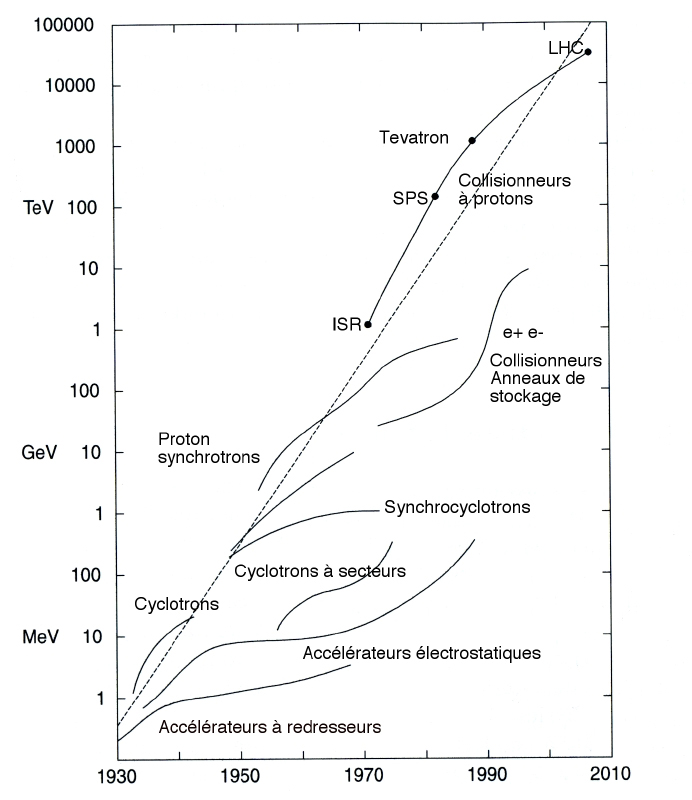
\includegraphics[width=0.8\textwidth]{LHC/Livingstone.jpg}
	\captionof{figure}{Diagramme de \bsc{Livingston} : énergie des faisceaux de particules accélérées pour différentes machines en fonction du temps. Afin de pouvoir comparer les différents accélérateurs et technologies, l'énergie des collisionneurs, qui s'exprime dans le centre de masse, a été recalculée comme si l'énergie des particules observées était le résultat d'une collision avec un proton au repos (cible fixe).}
	\label{livingston}	
\end{minipagewithmarginpars}

La figure \ref{lhcschema} est une vue schématique du LHC. En vérité le LHC n'est pas parfaitement circulaire, mais est composé d'octants (cf.Fig~\ref{octants}) qui comportent chacun une section droite de longueur \SI{528}{\meter} et un secteur courbe d'une longueur de \SI{2.45}{\kilo\meter}. 

\begin{minipagewithmarginpars}[ht!]{\textwidth}
	\centering
	\vspace*{1cm}
	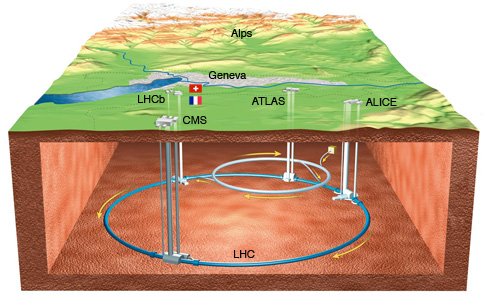
\includegraphics[scale=0.75]{LHC/CERNMap.jpg}
	\captionof{figure}{Vue schématique du LHC.}
	\label{lhcschema}	
\end{minipagewithmarginpars}

\begin{minipagewithmarginpars}[ht!]{0.95\textwidth}
	\centering
	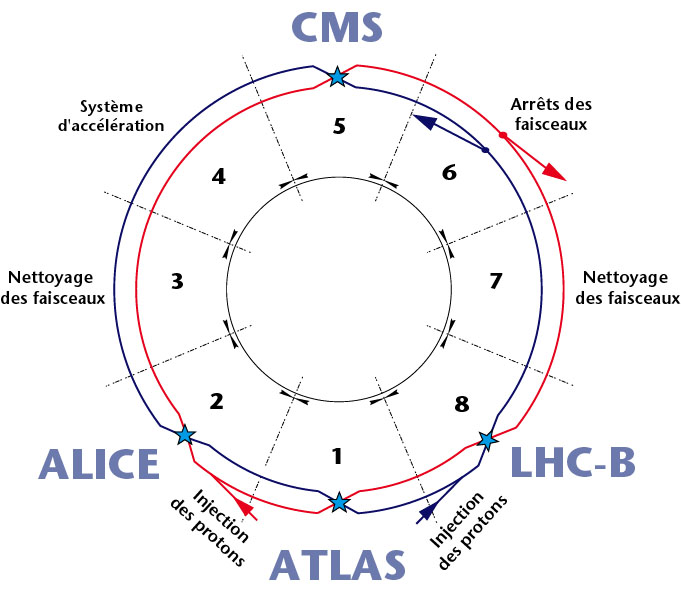
\includegraphics[width=0.80\textwidth]{LHC/lhc-schematic.jpg}
	\captionof{figure}{Vue schématique des octants du LHC ainsi que des positions des principaux détecteurs le long du LHC. Les faisceaux (en bleu et rouge) circulent en sens inverse l'un de l'autre.}
	\label{octants}	
\end{minipagewithmarginpars}

Afin de courber les faisceaux, \num{1232} aimants dipolaires de \num{15} mètres de long sont utilisés et \num{392} aimants quadripolaires de \num{5} à \SI{7}{\meter} permettent de concentrer les faisceaux. Chaque section courbe est composée de \num{23} cellules de \SI{106.9}{\meter} de long de type "FODO" (cf.Fig~\ref{fodo}).

\begin{minipagewithmarginpars}[ht!]{0.95\textwidth}
	\centering
	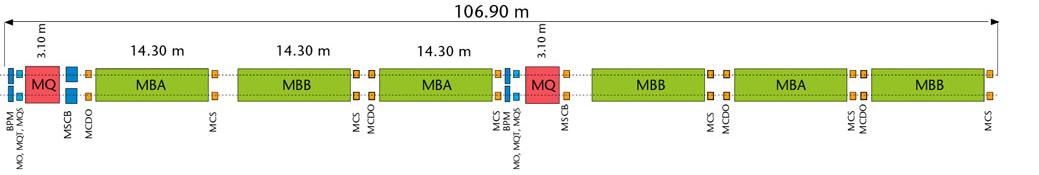
\includegraphics[width=0.8\textwidth]{LHC/arc.jpg}
	\captionof{figure}{Structure d'une cellule d'un octant.}
	\label{fodo}	
\end{minipagewithmarginpars}

\marginpar
{
	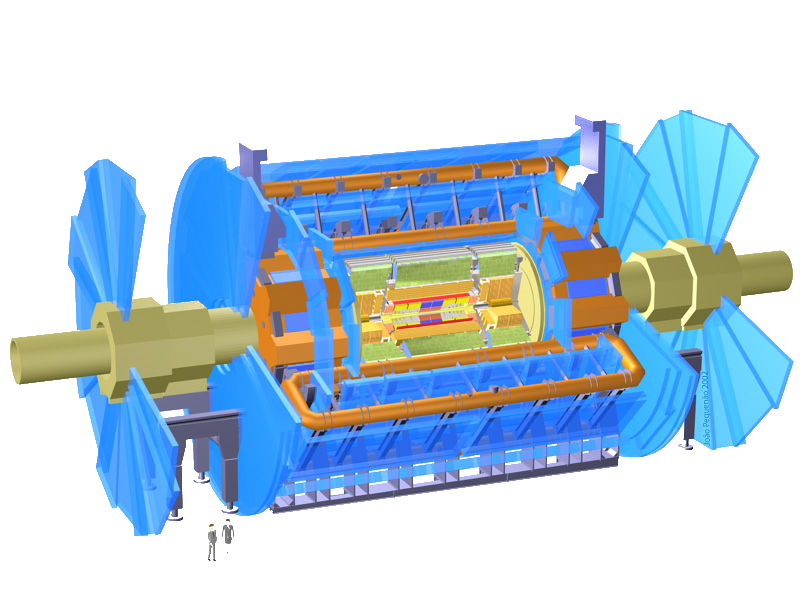
\includegraphics[width=\marginparwidth]{LHC/atlas.png}
	\captionof{figure}{ATLAS.}
	\label{atlas}
}

\marginpar
{
	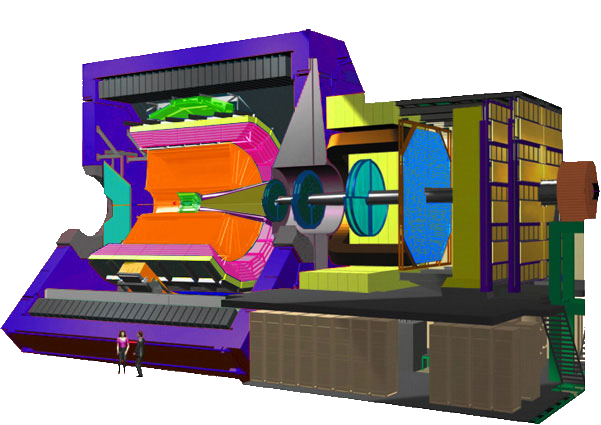
\includegraphics[width=\marginparwidth]{LHC/alice.png}
	\captionof{figure}{ALICE.}
	\label{alice}
}

\marginpar
{
	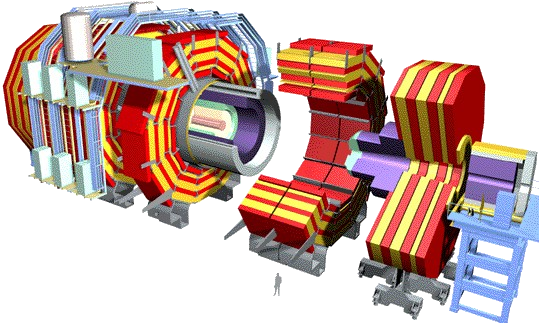
\includegraphics[width=\marginparwidth]{LHC/cms.png}
	\captionof{figure}{CMS.}
	\label{cms}
}

\marginpar
{
	
	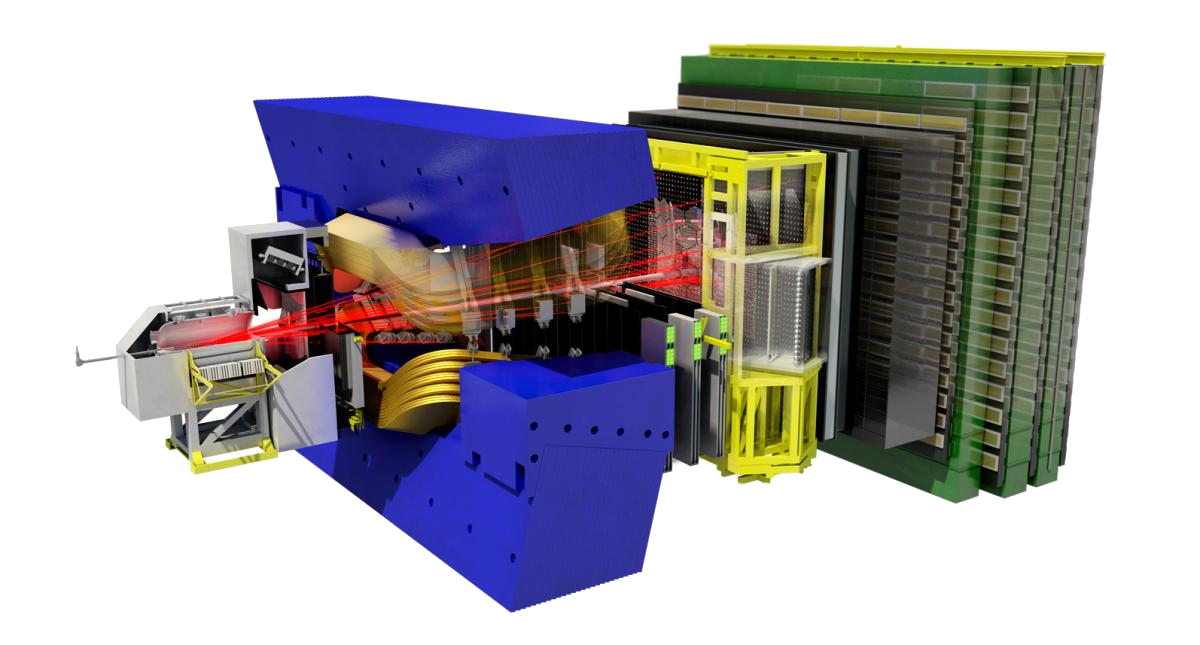
\includegraphics[width=\marginparwidth]{LHC/lhcb.png}
	\captionof{figure}{LHCb.}
	\label{lhcb}
}

\marginpar
{
	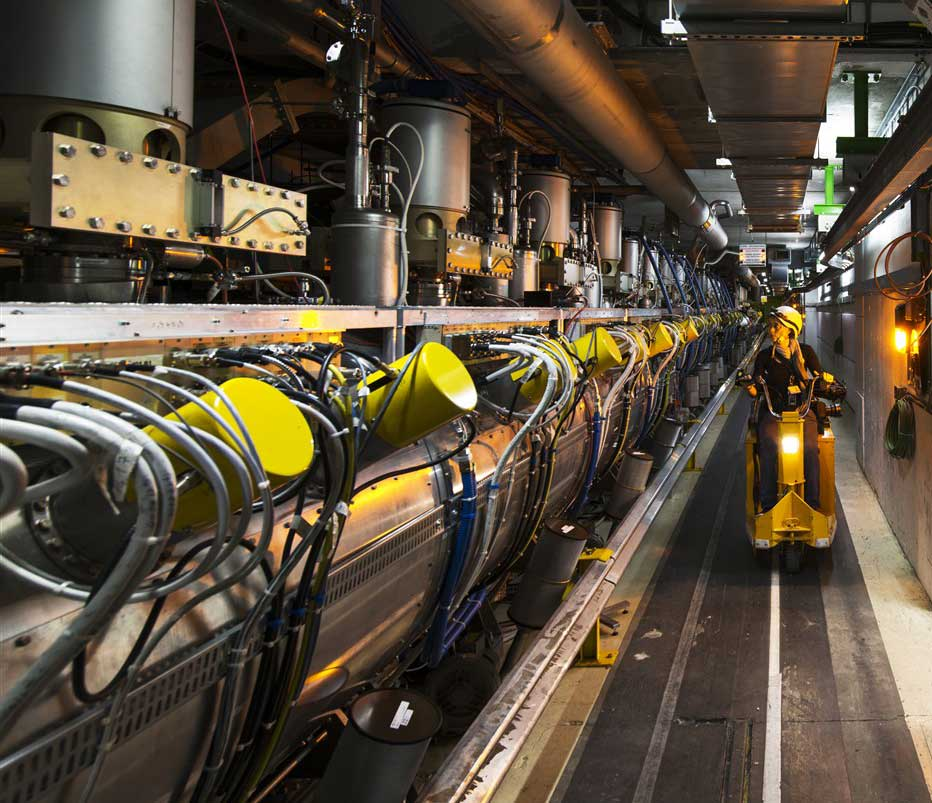
\includegraphics[width=\marginparwidth]{LHC/RF.jpg}
	\captionof{figure}{Photo d'une cavité accélératrice radiofréquence (RF).}
	\label{radio}
}

Deux quadrupôles MQ focalisent les faisceaux dans le plan vertical et horizontal respectivement, et six dipôles (MBA, MBB) courbent la trajectoire des particules. Les dipôles sont entourés de sextupôles, octopôles et décapôles afin de compenser les imperfections des champs magnétiques dipolaires. Des sextupôles, quadrupôles et octupôles sont également positionnés près des quadrupôles MQ afin de corriger les aberrations chromatiques.

Les sections droites sont utilisées afin de faire converger les deux faisceaux de protons venant en sens inverse l'un de l'autre. Il existe \num{8} points potentiels d'interactions (P), mais seulement \num{4} sont le siège de collisions et possèdent des détecteurs qui analysent les données issues de celles-ci : le point P1 pour ATLAS\footnote{A Toroidal LHC ApparatuS, détecteur généraliste.} (cf.Fig~\ref{atlas}), le point P2 pour ALICE\footnote{A Large Ion Collider Experiment, dédié à l'étude du plasma de quarks et gluons.}(cf.Fig~\ref{alice}), le point P5 pour CMS\footnote{Compact Muon Solenoid, détecteur généraliste.}(cf.Fig~\ref{cms}) et le point P8 pour LHCb\footnote{Large Hadron Collider beauty experiment, dédié au quark b.}(cf.Fig~\ref{lhcb}). Les sections droites des octants \num{3} et \num{7} contiennent des systèmes de nettoyage des faisceaux, le \num{6} un système d'arrêt des faisceaux et le \num{4} un système radiofréquence pour chaque faisceau (cf.Fig~\ref{radio}). Chaque système radiofréquence est composé de \num{8} cavités accélératrices. Ce sont des résonateurs électromagnétiques, opérant à \SI{400}{\mega\hertz}, qui accélèrent les particules et compensent l'énergie perdue par radiation synchrotron.

La réutilisation du tunnel du LEP et l'énergie des faisceau (\SI{7}{\tera\eV}) ont imposé l'utilisation d'aimants supraconducteurs produisant des champs magnétiques de \SI{8.4}{\tesla}. De plus l'utilisation de deux faisceaux de protons voyageant en sens inverse et l'espace limité dans le tunnel ont amené à la création d'un nouveau type d'aimant où les deux tubes contenant les deux faisceaux sont insérés dans un même cryostat (cf.Fig~\ref{dipole}).

\begin{minipagewithmarginpars}[ht!]{0.95\textwidth}
\centering
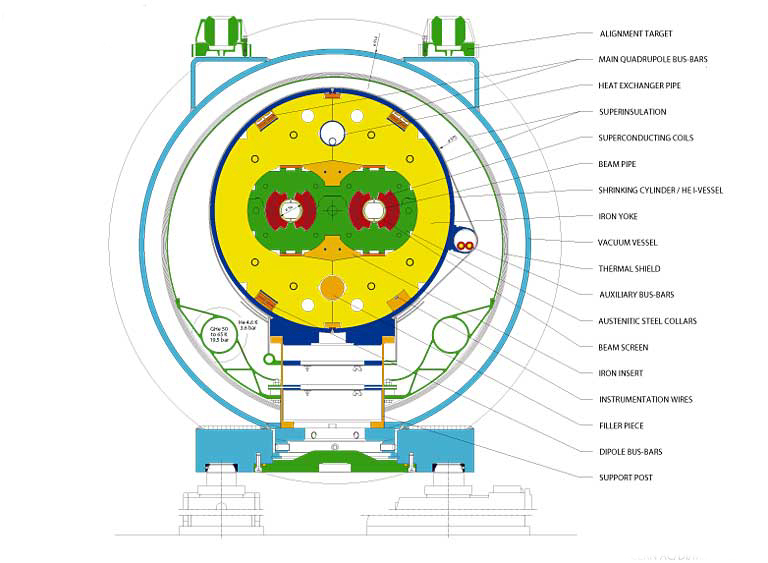
\includegraphics[width=1.0\textwidth]{LHC/dipole.jpg}
\captionof{figure}{Vue transversale d'un dipôle du LHC.}
\label{dipole}	
\end{minipagewithmarginpars}

\subsection{Luminosité des faisceaux}
Le nombre d'événements correspondant à un processus donné que peut produire le LHC peut être exprimé par :
\begin{equation}
N=\int \mathcal{L}(t)\sigma \mathrm dt
\end{equation}
où $\sigma$ est la section efficace du processus considéré (la probabilité qu'un événement produise ce processus), $t$ la durée de prise de données et $\mathcal{L}$ la luminosité instantanée délivrée par la machine.

La luminosité est déterminée par les paramètres des faisceaux de protons :
\begin{equation}
\mathcal{L}=\frac{f_{rev}n_{p}N_{f}}{4\pi \sigma_{x} \sigma_{y}} F(\phi)
\end{equation}
avec $N_{f}$ le nombre de protons par paquet, $n_{p}$ le nombre de paquets, $f_{rev}$ la fréquence de rotation d'un paquet, $\sigma_{x}$ ($\sigma_{y}$) la moyenne quadratique horizontale (verticale) transverse de la taille du faisceau au point d'interaction et $F(\phi)$ le facteur de réduction géométrique défini en fonction de l'angle $\phi$ de Piwinski.
\begin{equation}
F(\phi)=\frac{1}{\sqrt{1+\phi^{2}}}
\end{equation}
En considérant des faisceaux se croisant dans le plan vertical (cf.Fig~\ref{collision}), l'angle de Piwinski peut s'écrire :
\begin{equation}
\phi=\frac{\theta_{c}\sigma_{z}}{2\sigma_{y}}
\end{equation}
avec $\theta_{c}$ l'angle de croisement des faisceaux et $\sigma_{z}$ la moyenne quadratique de la longueur d'un paquet.


\begin{minipagewithmarginpars}[ht!]{0.95\textwidth}
\centering
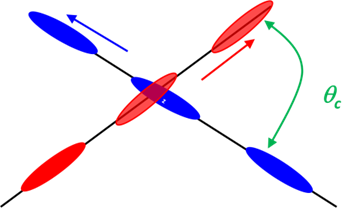
\includegraphics[width=0.45\textwidth]{LHC/collision.png}
\captionof{figure}{Schéma d'une collision de paquets dans le plan transversal.}
\label{collision}	
\end{minipagewithmarginpars}

Il est possible d'exprimer $\sigma_{x}$ et $\sigma_{y}$ en fonction de l'émittance $\epsilon$ et de la fonction $\beta(s)$, avec $s$ la position le long de la trajectoire nominale du faisceau. L'émittance est l'espace dans l'espace des phases qui contient un certain pourcentage des particules du faisceau (\num{95}\% pour les collisionneurs hadroniques). Elle est supposée constante durant toute la durée du temps de mesure \footnote{d'après le théorème de \bsc{Liouville}.} :
\begin{equation}
\sigma_{x}=\sqrt{\epsilon\beta_{x}}
\end{equation}

La valeur de la fonction $\beta$ au point d'interaction est notée $\beta^{*}$. En considérant de plus que $\sigma_{x}=\sigma_{x}=\sigma$ on peut réécrire $\mathcal{L}$ comme :
\begin{equation}
\mathcal{L}=\frac{f_{rev}\gamma\beta n_{p}N_{f}}{4\epsilon_{n}\beta^{*}\pi} F(\phi)
\end{equation}
où $\epsilon_{n}=\epsilon\gamma\beta$ est l'émittance normalisée et $\gamma$ le facteur de \bsc{Lorentz} $\beta=v/c$.

\newpage
D'après cette formule on remarque qu'il peut être intéressant de réduire au maximum $\epsilon_{n}$ c'est-à-dire d'avoir des paquets dont les particules ont la même quantité de mouvement et sont proches l'une de l'autre. Il est aussi possible de diminuer le facteur de réduction géométrique en utilisant une configuration de faisceau dite "en crabe" (cf.Fig~\ref{crabe})

\begin{minipagewithmarginpars}[ht!]{0.95\textwidth}
\centering
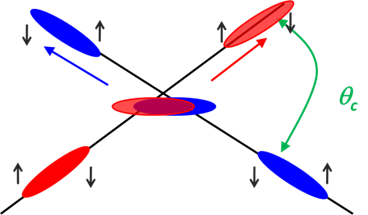
\includegraphics[width=0.45\textwidth]{LHC/crab.png}
\captionof{figure}{Schéma d'une collision "en crabe" de paquets dans le plan transversal.}
\label{crabe}	
\end{minipagewithmarginpars}

La luminosité du faisceau ne reste pas constante tout le long d'un cycle de prise de données. Les collisions dans les détecteurs en sont la cause principale. Le temps de décroissance caractéristique de l'intensité du faisceau par les collisions est :
\begin{equation}
\tau_{collisions}=\frac{N_{0}}{L_{0}\sigma_{tot}n}
\end{equation}
avec $N_{0}$ le nombre de protons à l'injection, $L_{0}$ la luminosité initiale, $\sigma_{tot}$ la section efficace totale et $n$ le nombre de points d'interaction des faisceaux.

Les deux autres causes principales de la réduction de la luminosité des faisceaux sont, d'une part la perte par interaction entre les particules du faisceau et le gaz piégé dans les tubes (avec un temps caractéristique $\tau_{gaz}$), d'autre diverses perturbations et imperfections (champ magnétique par exemple) qui peuvent dévier les particules de la trajectoire nominale du faisceau ($\tau_{imper}$). 
La décroissance de la luminosité instantanée peut être donnée par la formule:
\begin{equation}
\frac{\mathrm \mathcal{L}}{\mathrm t} = L_{0} e^{-\frac{t}{\tau}}
\end{equation}
avec
\begin{equation}
\frac{1}{\tau} = \frac{1}{\tau_{collisions}}+\frac{1}{\tau_{gaz}}+\frac{1}{\tau_{imper}}
\end{equation}

Lorsque l'intensité du faisceau devient trop faible pour une prise de données efficace, les faisceaux sont déviés de leurs trajectoires circulaires et envoyés dans les "\textit{dump blocks}" (cf.Fig~\ref{dump})
\marginpar
{
	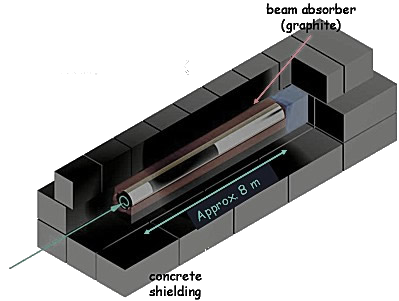
\includegraphics[width=\marginparwidth]{LHC/dump.png}
    \captionof{figure}{Schéma d'un \textit{"dump block"}.}
    	\label{dump}
}

La luminosité intégrée pour les collisions proton-proton délivrées par le LHC en \num{2016} ainsi que celle enregistrée par le détecteur CMS sont données par le graphique suivant :

\begin{minipagewithmarginpars}[ht!]{0.95\textwidth}
\centering
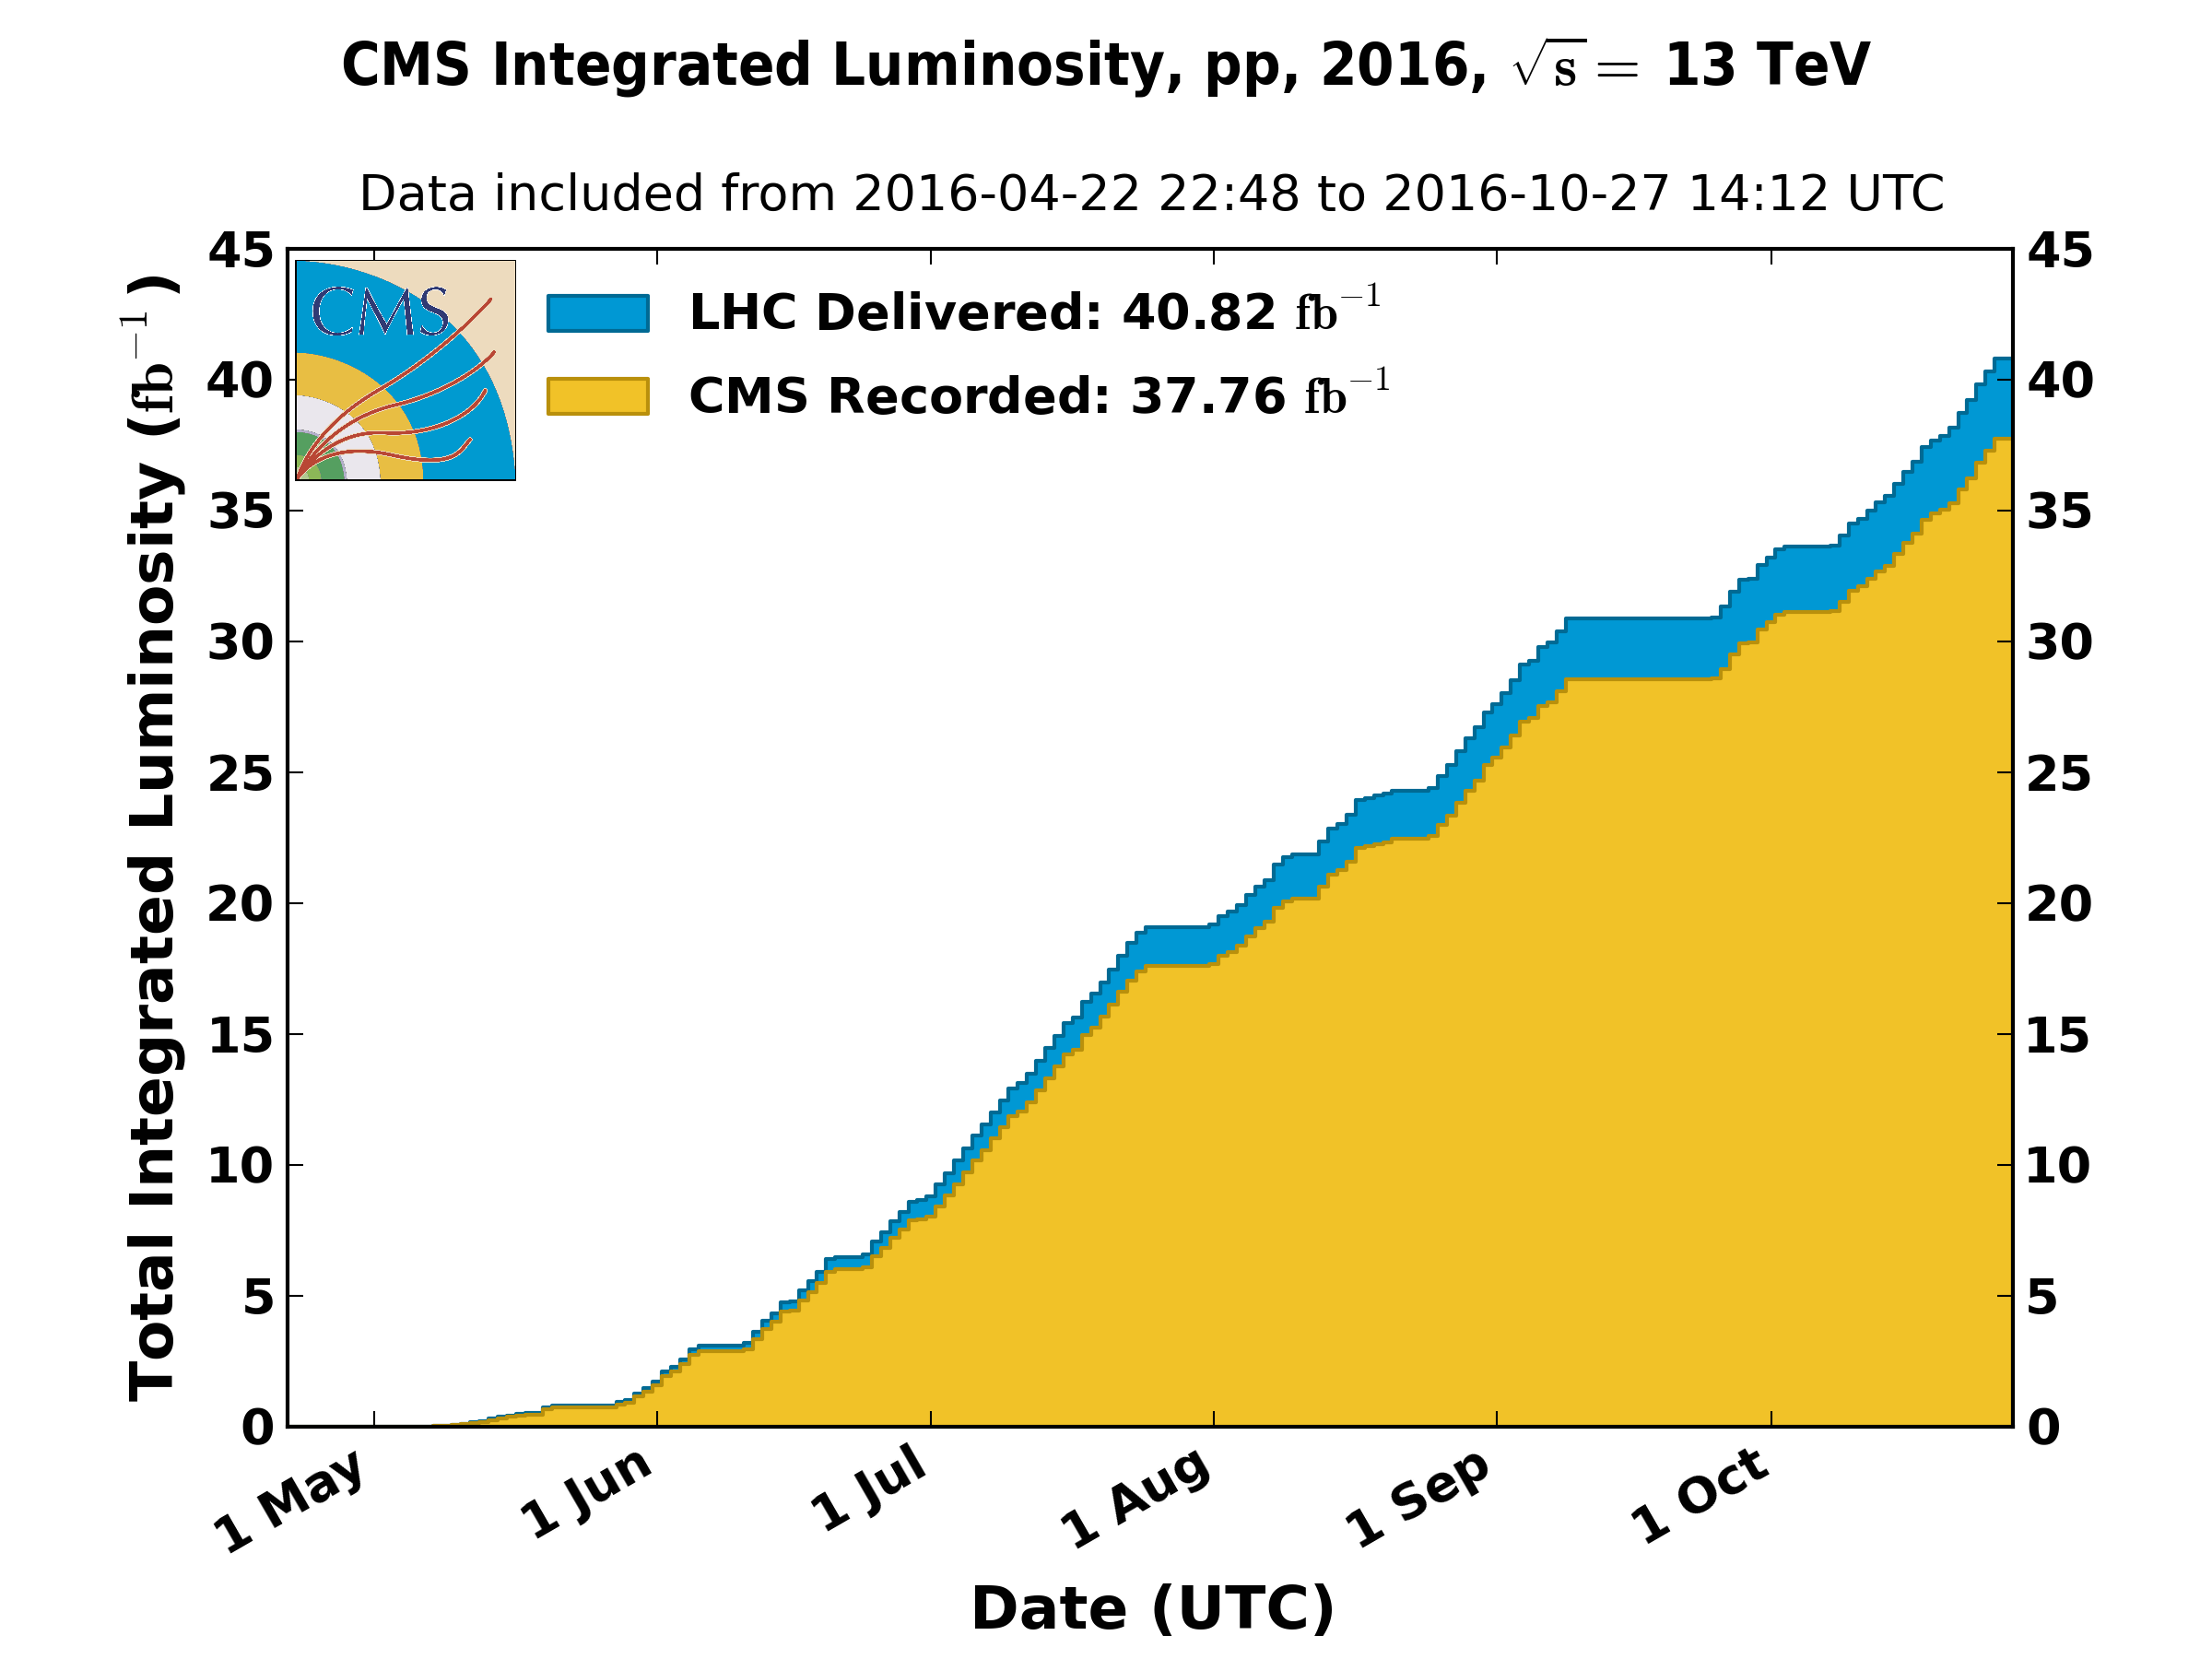
\includegraphics[width=0.50\textwidth]{LHC/luminosity.png}
    \captionof{figure}{Luminosité intégrée en fonction du jour de l'année \num{2016} délivrée (bleu) et enregistrée (orange) par CMS pendant les faisceaux stables et pour les collisions $pp$, à \SI{13}{\tera\eV} d'énergie dans le centre de masse \cite{lumipileup}.}
\end{minipagewithmarginpars}

\subsection{Collisions proton-proton}
Le proton n'est pas une particule élémentaire. Il est composé de \num{3} quarks de valence ($uud$) et de quarks, antiquarks et gluons regroupés sous le terme de partons (cf.Fig~\ref{proton})

\begin{minipagewithmarginpars}[ht!]{0.95\textwidth}
\centering
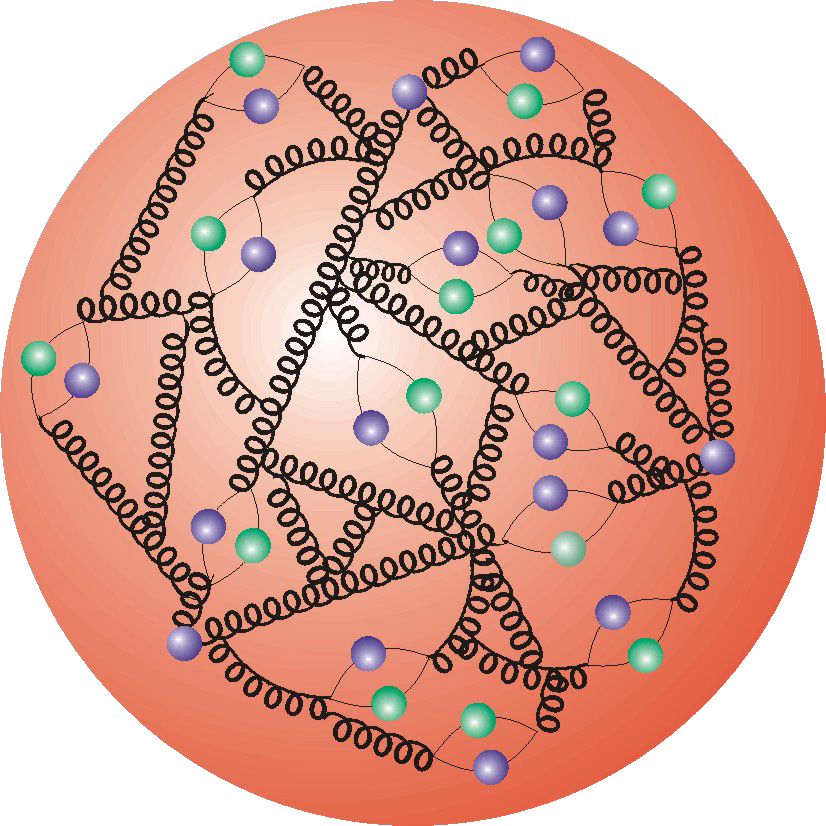
\includegraphics[width=0.3\textwidth]{SM/quarks3.png}
\captionof{figure}{Schéma d'un proton : les quarks (vert) et anti-quarks (bleu) sont en interaction par l'intermédiaire de gluons (noir).}
\label{proton}	
\end{minipagewithmarginpars}

Les collisions proton-proton peuvent être rassemblées en trois groupes :
\begin{itemize}[label=$\bullet$]
	\item \textbf{Les collisions élastiques : } elles préservent l'énergie cinétique totale des protons. Ces collisions ne sont pas intéressantes dans notre cas et ne font que polluer. Elles correspondent à des collisions de faible quantité de mouvement.
	\item\textbf{Les collisions diffractives : } elles se produisent lorsque la quantité de mouvement des deux protons et plus importante. Elles se caractérisent par la fragmentation d'un proton pour la diffraction simple ou des deux protons pour la diffraction double.
	\item \textbf{Les collisions inélastiques : } ces collisions se produisent lorsque l'un des partons d'un proton interagit avec un parton de l'autre proton. Ce sont ces interactions à haute quantité de mouvement qui sont les plus intéressantes pour la recherche de nouvelle particules.
\end{itemize}

\subsubsection{Collisions inélastiques}
Les collisions inélastiques se produisent entre deux partons qui possèdent une fraction de la quantité de mouvement $x_{1}$ et $x_{2}$ du proton $1$ et $2$. Ces fractions sont décrites par des fonctions de distribution de partons $f(x,Q^{2})$. Il s'agit des densités de probabilités de trouver une particule avec une fraction $x$ de la quantité de mouvement longitudinale du hadron dont l'impulsion est $Q^{2}$. Il existe une fonction de distribution de parton par saveur de quark et une pour les gluons (cf.Fig~\ref{pdf}).

\begin{minipagewithmarginpars}[ht!]{0.95\textwidth}
	\centering
	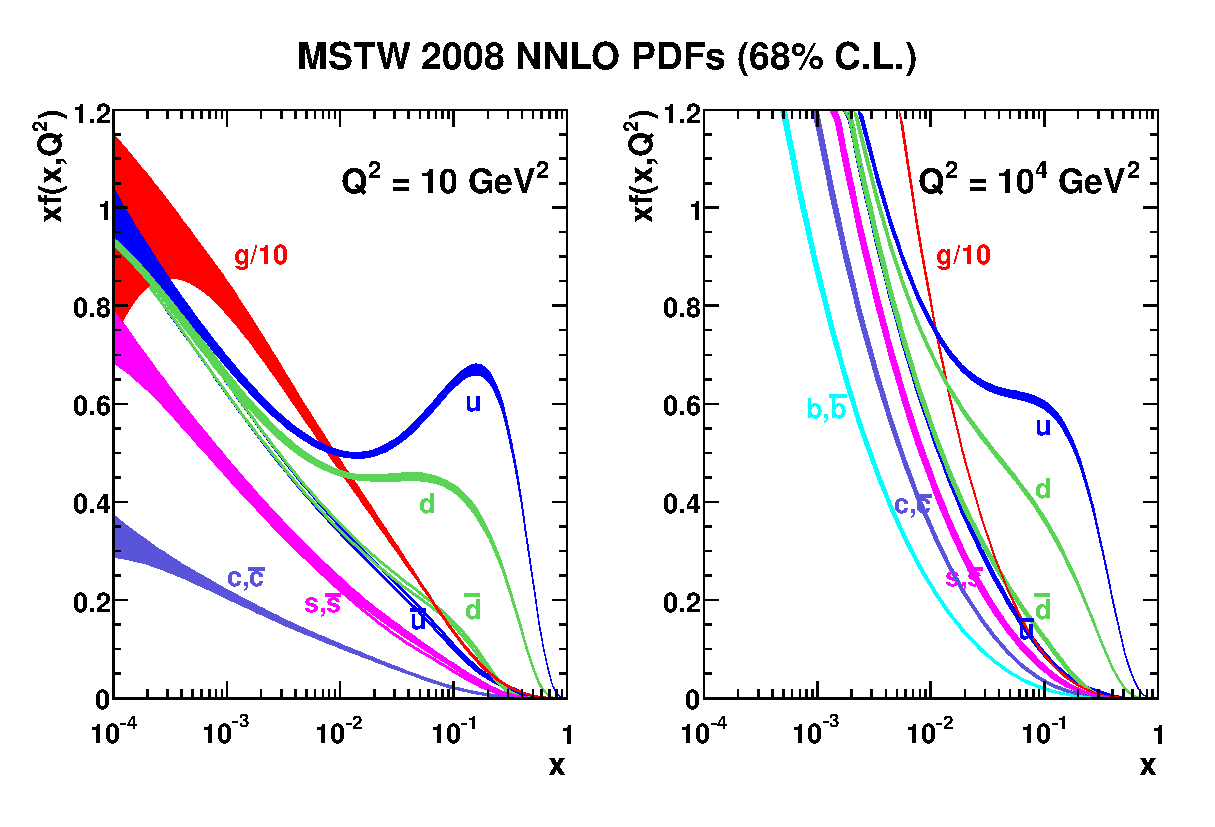
\includegraphics[width=0.6\textwidth]{LHC/pdf.eps}
	\captionof{figure}{Produit de $x$ avec la  distribution de parton non-polarisée $f(x)$, où $f=u$, $\bar{u}$, $d$, $\bar{d}$, $c$, $\bar{c}$, $s$, $\bar{s}$, $b$, $\bar{b}$, $g$ et leurs incertitudes, en utilisant la paramétrisation NNLO MSTW2008 à l'échelle \SI{10}{\square\giga\eV} (gauche) et \SI{10000}{\square\giga\eV} (droite) \cite{Martin:2009iq}.}
	\label{pdf}	
\end{minipagewithmarginpars}
 
Ces fonctions ne peuvent être déduites que des données expérimentales car l'échelle d'énergie de QCD à laquelle sont soumis les partons au sein du proton ne permet pas d'effectuer un calcul perturbatif. On peut remarquer que la contribution des gluons est la plus importante et que les quarks de valence ont une contribution plus importante que ceux de la mer de partons.

En utilisant ces fonctions et le théorème de factorisation de QCD, il est possible de calculer la section efficace d'un événement $A+B\rightarrow X$ par la formule :
\begin{equation}
\sigma_{A+B\rightarrow X}=\sum_{i=q,g}\int_{0}^{1} \mathrm{d}x_{a}\mathrm{d}x_{b}f_{a/A}(x_{a},\mu_{F}^{2})f_{b/B}(x_{b},\mu_{F}^{2})\sigma{_{a+b\rightarrow X}}
\end{equation}
L'échelle de factorisation $\mu^{2}$ est la limite entre la partie non perturbative $f_{b/B}(x_{b},\mu^{2})$ et la partie calculable par la théorie perturbative de la section efficace $\sigma{_{a+b\rightarrow X}}$.

Il est ainsi possible de calculer $\sigma{_{a+b\rightarrow X}}$ par la méthode perturbative et de la développer en termes de puissance de la constante de couplage $\alpha_{s}\left(\mu_{R}^{2}\right)$ qui dépend de l'échelle de renormalisation:
\begin{equation}
\sigma_{a+b\rightarrow X}=\left[\sigma_{0}+\alpha_{s}\left(\mu_{R}^{2}\right)\sigma_{1}+\cdots\right]_{a+b\rightarrow X}
\label{eq2}
\end{equation}
La figure \ref{crosssection} montre quelques sections efficaces du Modèle Standard pour des collisions proton-proton et proton-anti-proton calculées au \textit{"next-to-leading order"} ($\sigma_{1}$ dans la formule \ref{eq2}).

\begin{minipagewithmarginpars}[ht!]{0.95\textwidth}
	\centering
	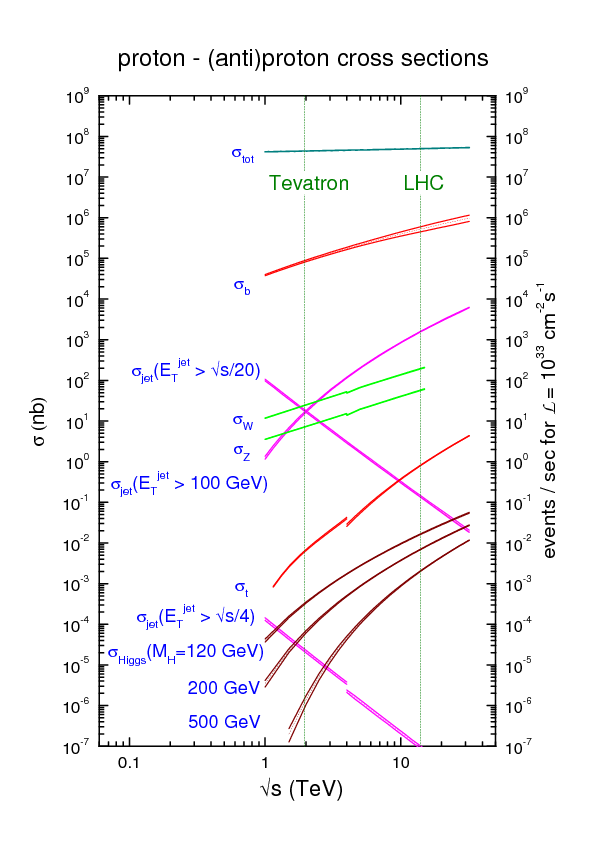
\includegraphics[width=0.60\textwidth]{LHC/crosssections2008.png}
	\captionof{figure}{Sections efficaces du Modèle Standard pour les collisionneurs LHC et Tevatron en fonction de l'énergie dans le centre de masse $\sqrt{s}$. Les lignes pointillées indiquent les énergies dans le centre de masse associées au Tevatron (\SI{1.96}{\tera\eV}) et au LHC (\num{7}, \num{10} et \SI{14}{\tera\eV}). Les sections efficaces sont exprimées en nanobarn (gauche) et en Hertz (droite) pour une luminosité instantanée $\mathrm{L}=$\SI{e33}{\per\square\centi\meter\per\second}, luminosité typique des premières années de fonctionnement du LHC \cite{sectioneff}.}
	\label{crosssection}	
\end{minipagewithmarginpars}

\subsection{Collisions proton-proton inélastiques}
Les collisions inélastiques sont le siège de plusieurs processus (cf.Fig~\ref{collision2}). Parmi les plus importants citons :
\begin{itemize}[label=$\bullet$]
	\item \textbf{Les collisions profondément inélastiques :} deux partons très énergétiques des deux protons entrent en collision.
	\item \textbf{Les collisions sous-jacentes :} plusieurs collisions entre les partons restant des protons peuvent avoir lieu.
	\item \textbf{Les radiations de l'état initial :} avant l'interaction des deux partons responsables de la collision principale, ces deux partons peuvent rayonner des quarks et des gluons.
	\item \textbf{Les radiations finales :} les particules créées après la collision principale peuvent elles-mêmes rayonner des quarks et des gluons.
	\item \textbf{L'hadronisation :} due à la propriété de confinement, les quarks et gluons vont s'hadroniser afin de former des hadrons de couleur blanche qui forment des jets.
	\item \textbf{Les désintégrations :} nombre des hadrons et mésons créés pendant le processus d'hadronisation ne sont pas stables et vont se désintégrer, parfois en cascade, en particules stables.
\end{itemize}

\begin{minipagewithmarginpars}[ht!]{0.95\textwidth}
	\centering
	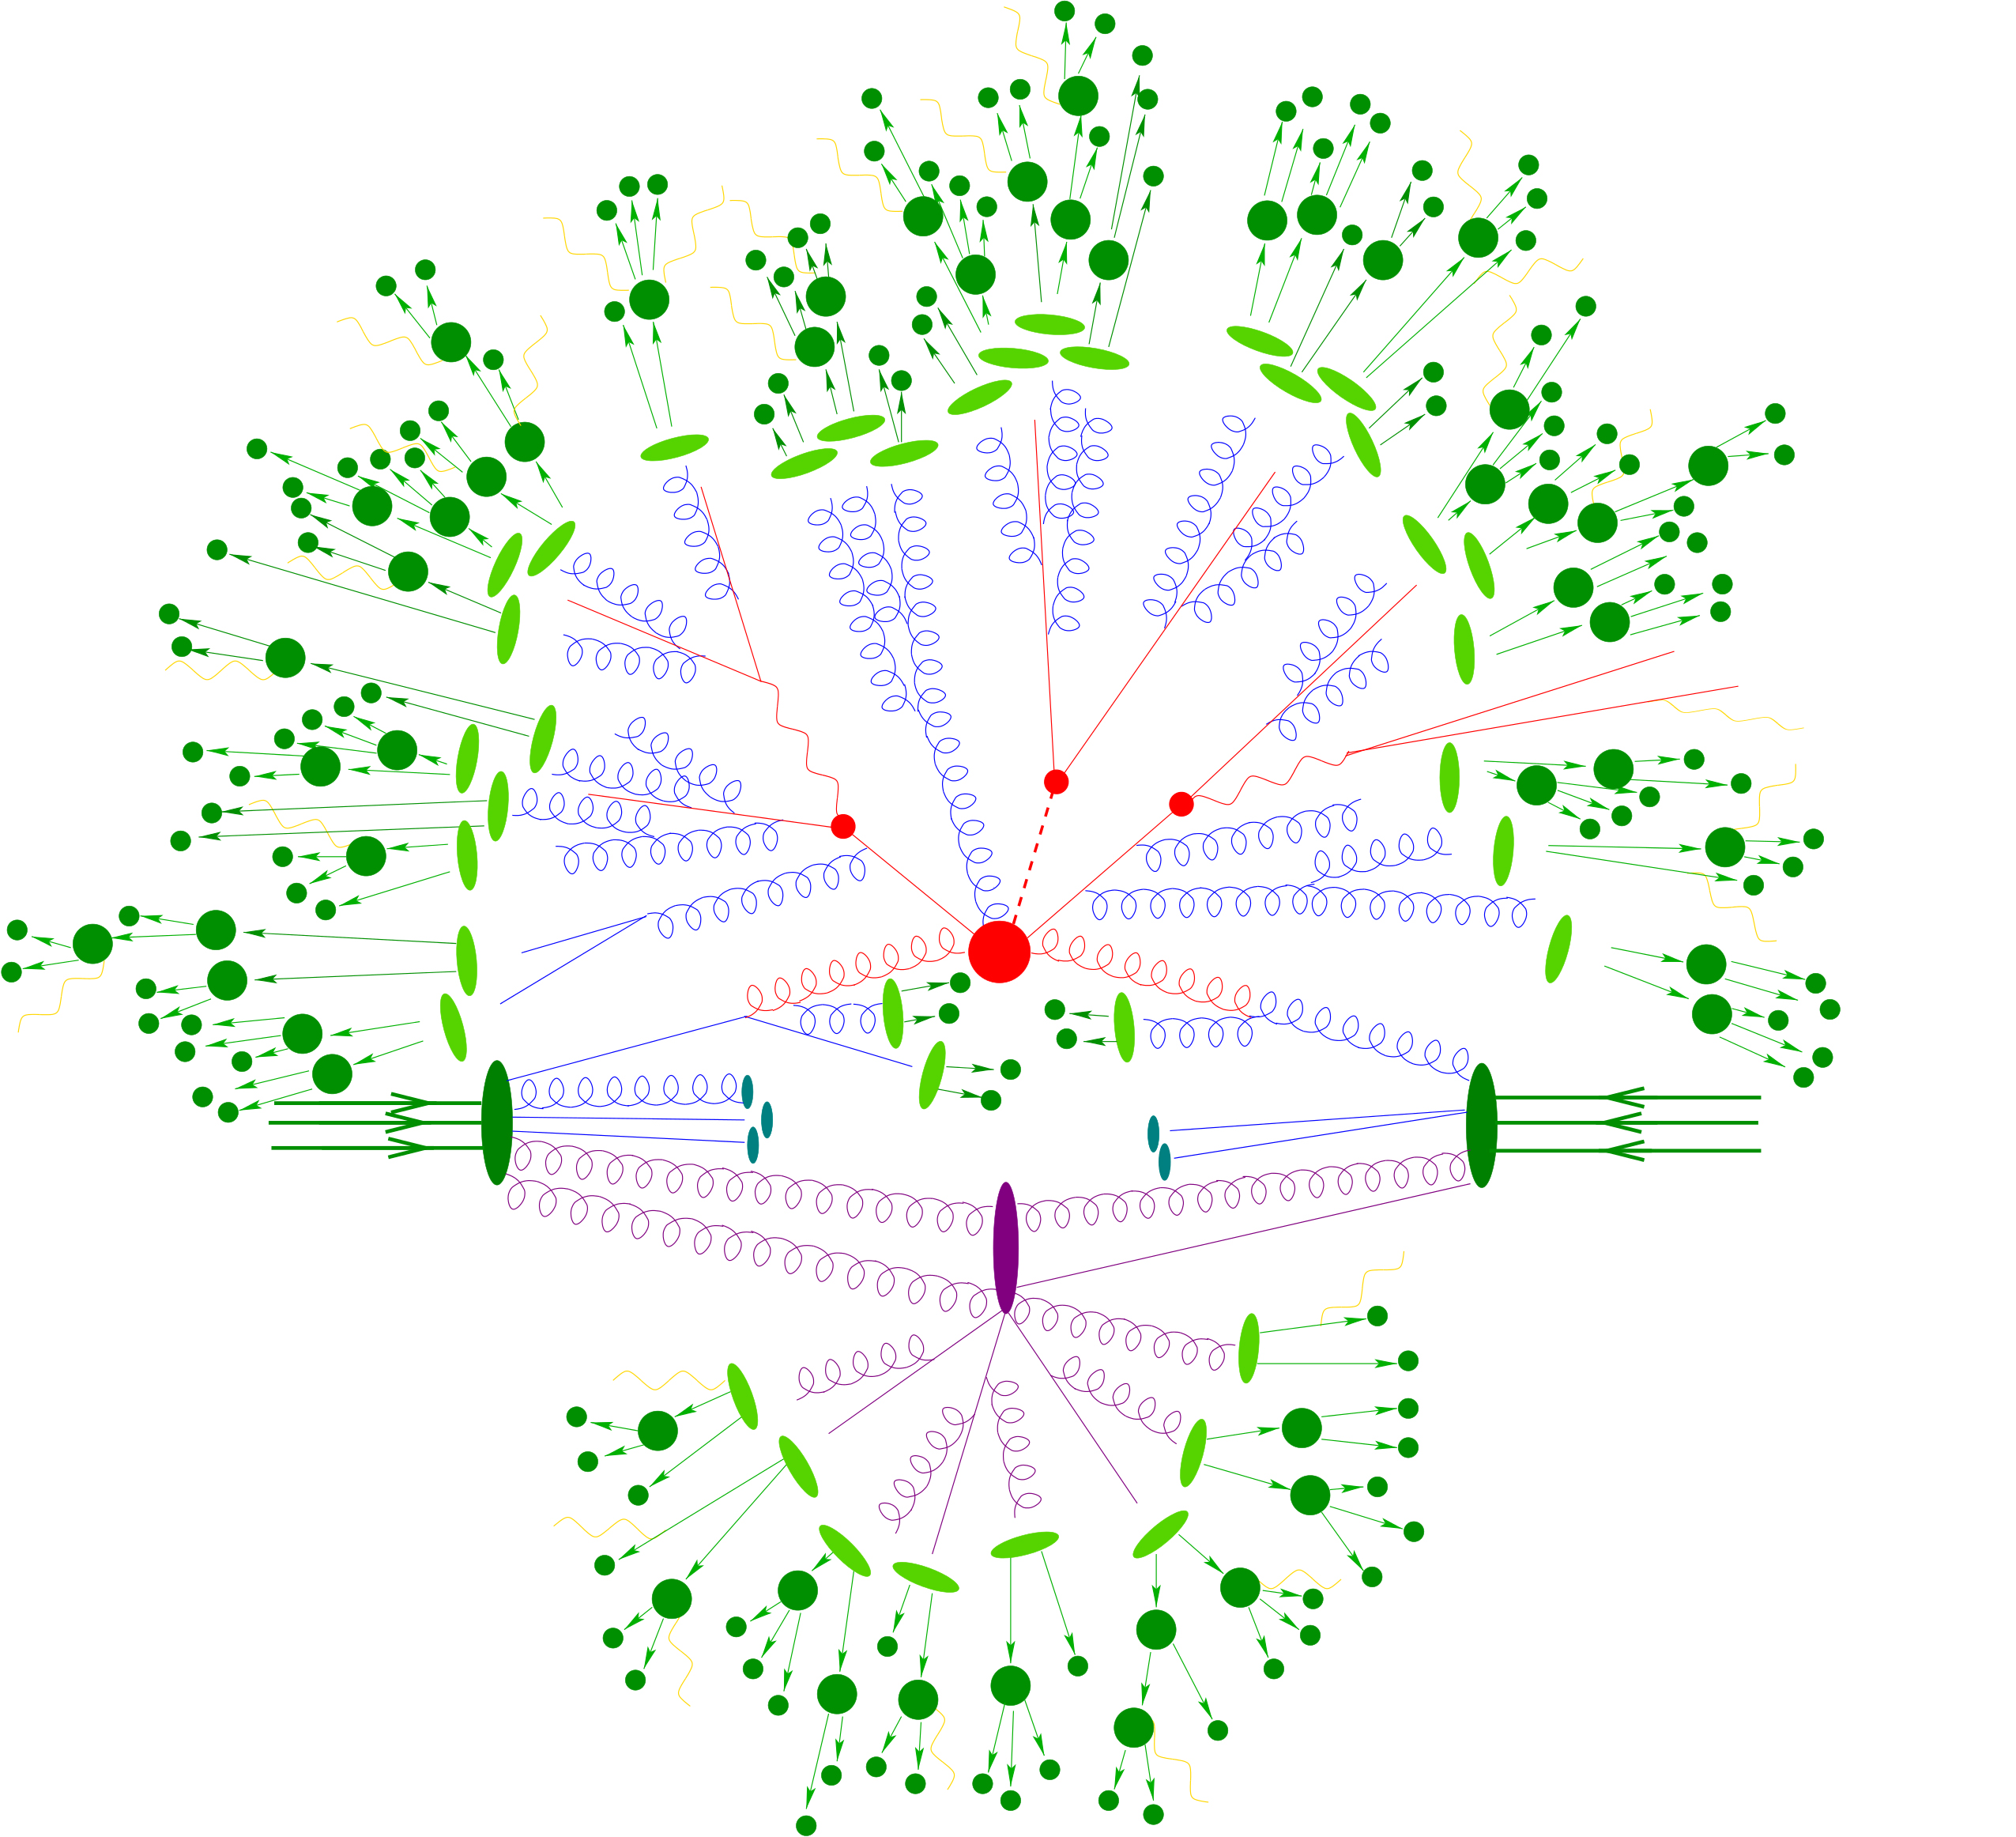
\includegraphics[width=1.0\textwidth]{LHC/event.jpg}
	\captionof{figure}{Schéma d'une collision proton-proton inélastique. Deux partons venant de deux protons différents interagissent inélastiquement (rouge), d'autres partons de ces deux protons produisent des collisions secondaires (magenta). Les partons ainsi créés s'hadronisent (rouge) en créant des jets de particules (vert clair). Ces particules instables se désintègrent, en cascade, en particules stables (vert foncé).}
	\label{collision2}	
\end{minipagewithmarginpars}

\subsection{L'empilement en temps et hors-temps}
Plusieurs collisions proton-proton peuvent avoir lieu lors d'un même croisement de faisceaux. Ces collisions appartiennent donc au même événement et forment un empilement en temps ou "\textit{on-time pile-up}". De plus certaines désintégrations et phénomènes peuvent durer plus longtemps que le temps entre deux croisements de faisceaux. Ces événements sont appelés empilement hors-temps ou "\textit{off-time pile-up}". Le phénomène d'empilement dépend de la luminosité et de l'énergie des faisceaux. La figure \ref{pile-up} montre la distribution du nombre d'événements par croisement de faisceaux dans CMS en \num{2012}.

\begin{minipagewithmarginpars}[ht!]{0.95\textwidth}
	\centering
	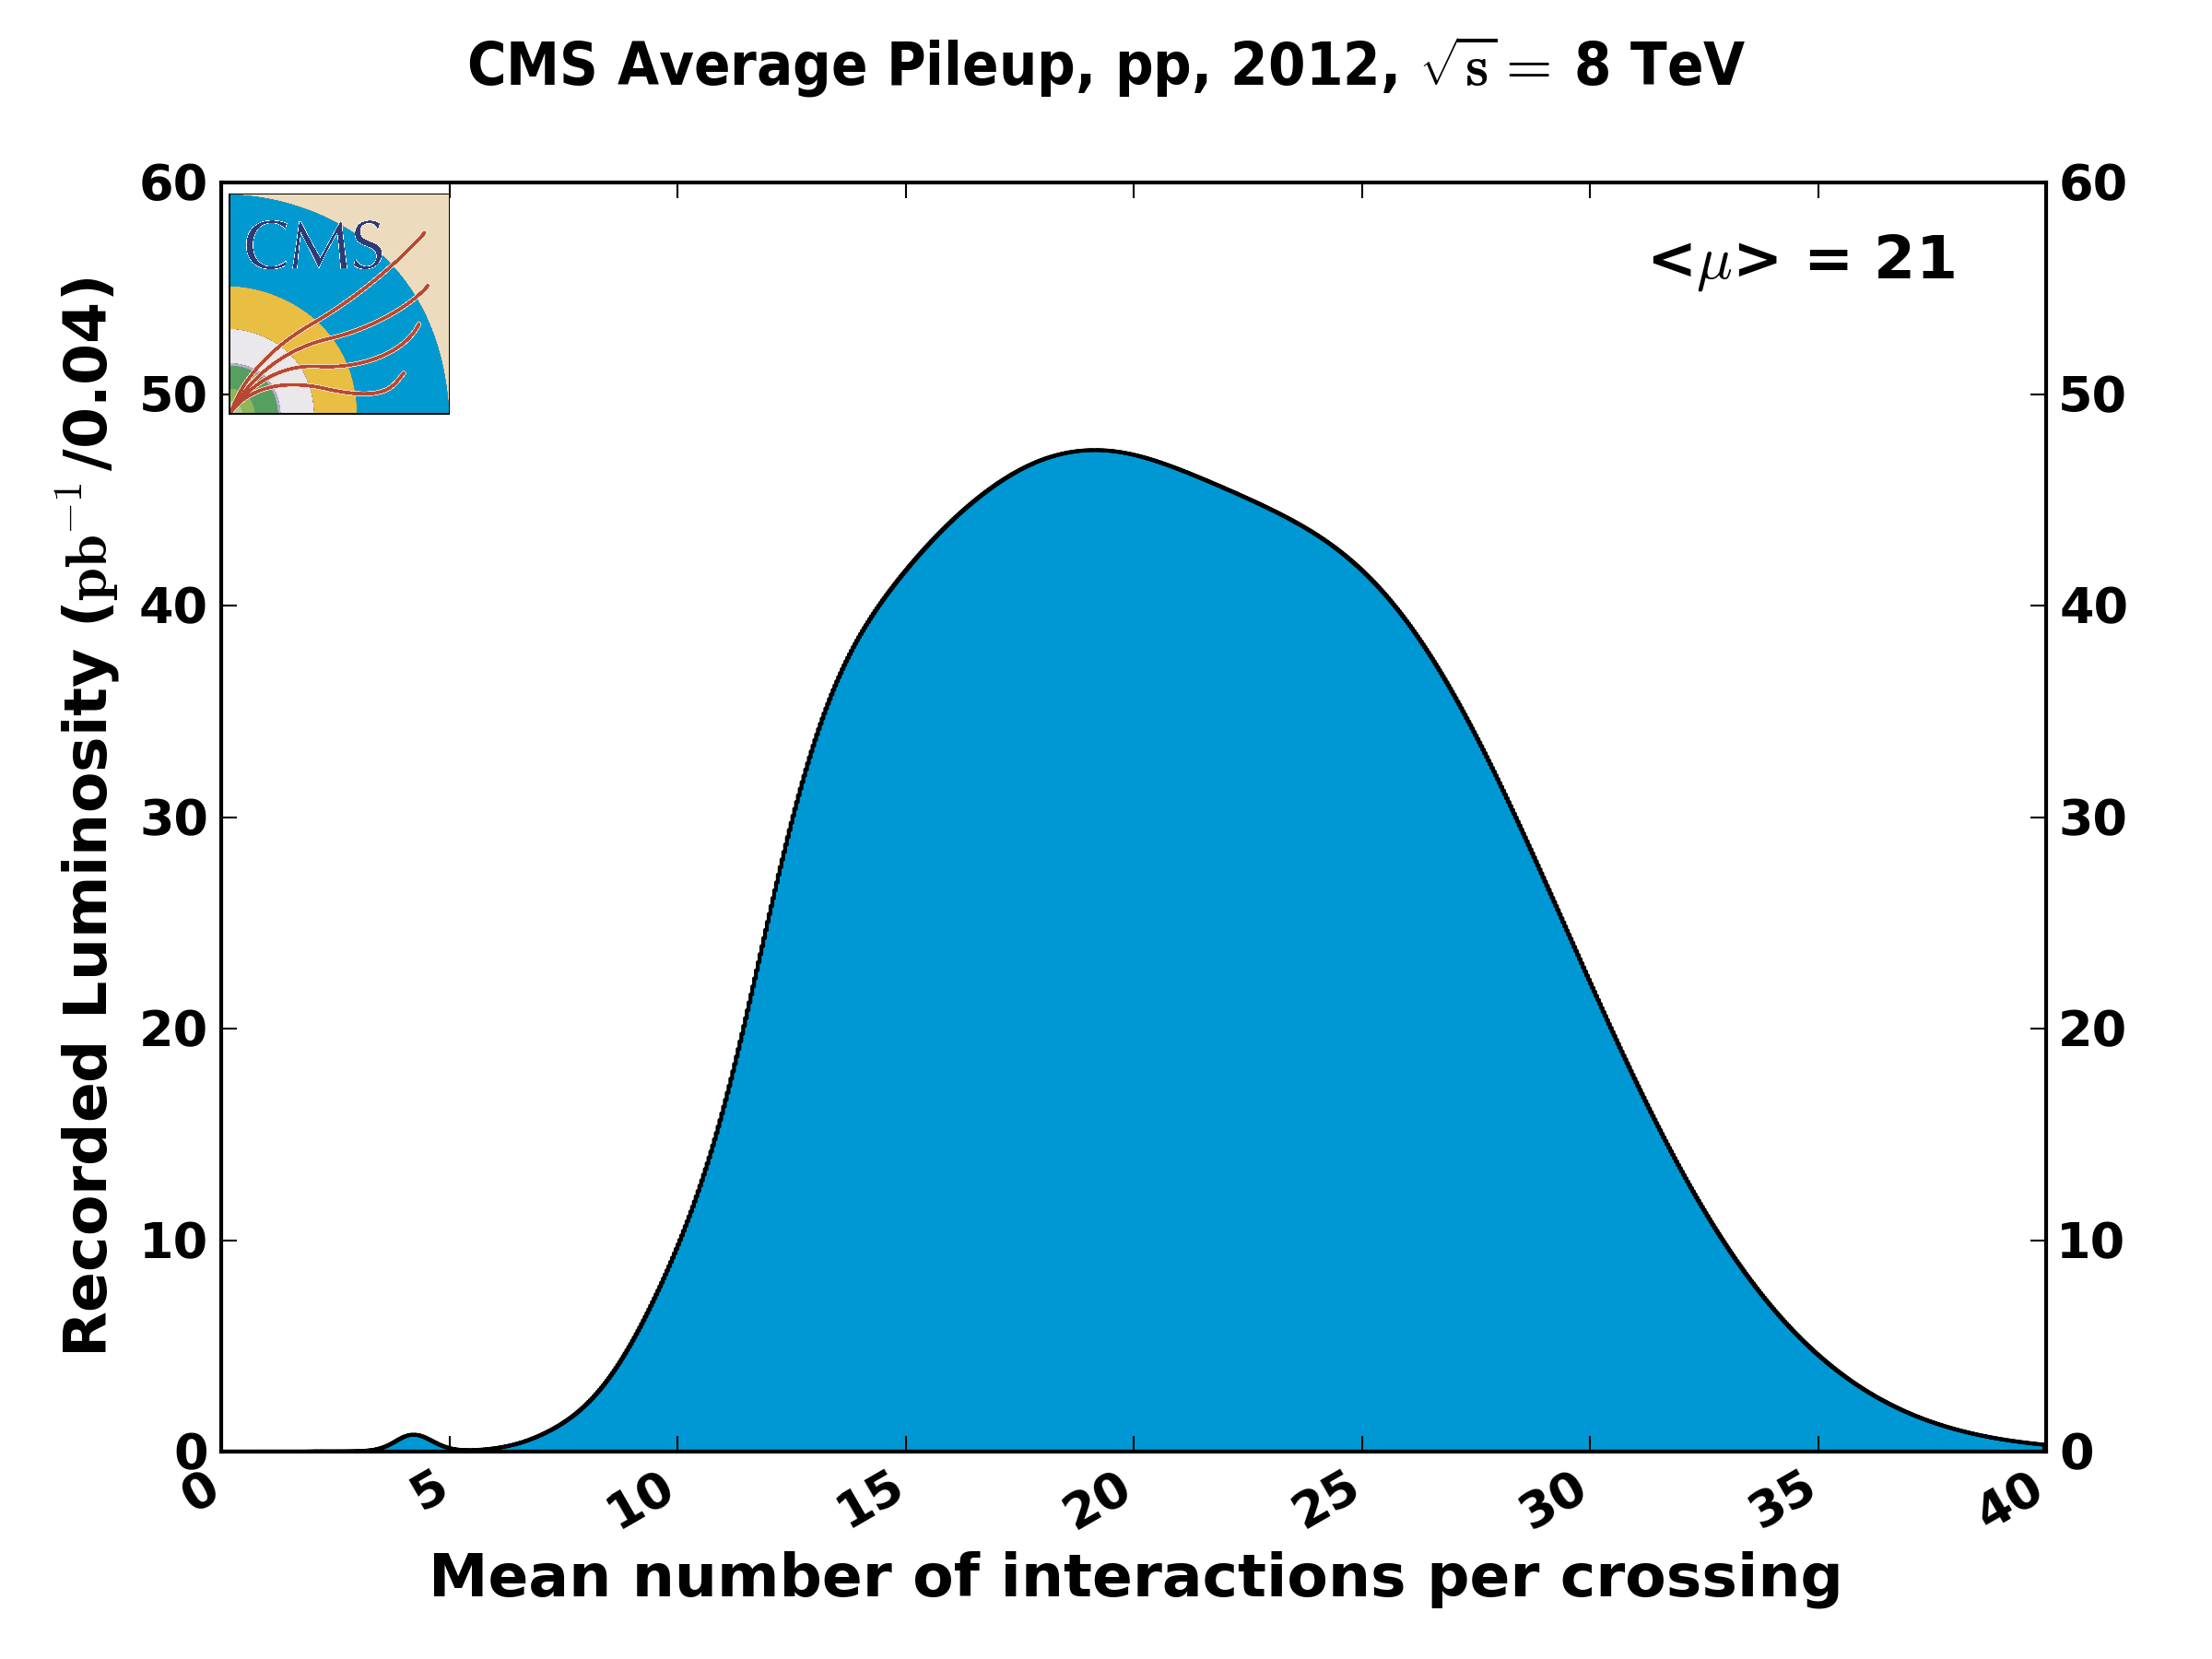
\includegraphics[width=0.60\textwidth]{LHC/pileup.png}
	\captionof{figure}{Distribution du nombre de collisions par croisement de faisceaux \cite{lumipileup}.}
	\label{pile-up}	
\end{minipagewithmarginpars}

\subsection{Vers le High Luminosity LHC (HL-LHC)}
De par l'envergure de la machine, du nombre d'expériences nécessitant le bon fonctionnement du LHC et du nombre de personnes impliquées dans ce projet, celui-ci a fait l'objet d'un calendrier prévisionnel (cf.Fig~\ref{roadmap}). Ce calendrier est divisé en deux grandes phases : la \textbf{Phase I} (\num{2010}--\num{2023}) et la  \textbf{Phase II} (\num{2023}--\num{2035}). Chacune d'elles est elle-même divisée en plusieurs périodes comportant des arrêts techniques et des arrêts beaucoup plus long appelés "\textit{Long Shut-down}" (LS). Ceux-ci permettent d'améliorer le LHC ainsi que d'avoir accès aux détecteurs à des fins de maintenances et d'améliorations. L'arrêt le plus important à venir est le LS3. Il est censé durer une trentaine de mois et permettre la mise à niveau du LHC vers le HL-LHC.

\begin{minipagewithmarginpars}[ht!]{0.95\textwidth}
	\centering
	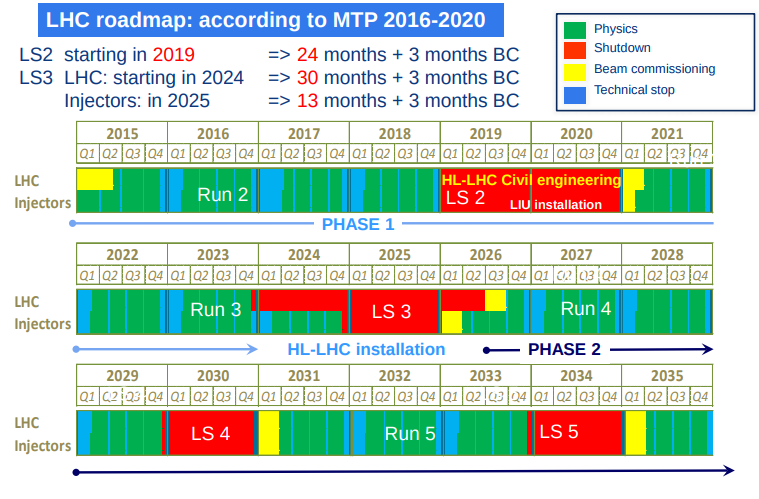
\includegraphics[width=0.80\textwidth]{LHC/roadmap.png}
	\captionof{figure}{Calendrier prévisionnel du LHC.}
	\label{roadmap}	
\end{minipagewithmarginpars}

\subsubsection{Le HL-LHC}
La mise à niveau du LHC en HL-LHC vise à multiplier la luminosité nominale par un facteur \num{5} à \num{7.5}.

Le but est de produire environ \num{140} événements de \textit{pile-up} par croisement de faisceaux contre une vingtaine actuellement. Pour cela les faisceaux devront être plus intenses et plus concentrés qu'actuellement. Afin d'y parvenir de nombreux paramètres du collisionneur et de la chaine d'accélération vont modifiés (cf.Fig~\ref{man}).

\begin{itemize}[label=$\bullet$]
	
 \item Un nouveau système optique est à l'étude afin d'adapter la concentration du faisceau au cours du temps pour maintenir une luminosité constante tout le long de la durée de vie du faisceau. D'autres instruments de mesures des paramètres des faisceaux seront également installés.
 
 \item Des aimants de \SI{12}{\tesla}, contre \SI{8}{\tesla} pour le présent système, seront installés à l'avant de ATLAS et CMS afin de mieux collimer les faisceaux.
 
 \item Des cavités supraconductrices vont être installées en vue d'orienter les paquets de particules en leur donnant un moment transverse afin d'augmenter la section efficace. Cette configuration est dite "en crabe".
 
 \item L'accroissement du nombre de particules nécessite un renforcement des protections afin de ne pas abîmer la machine. \num{60} des \num{118} collimateurs qui permettent l'absorption des particules qui s'échappent de la trajectoire nominale du faisceau seront remplacés et entre \num{15} et \num{20} nouveaux collimateurs seront installés.
 
 \item Afin d'insérer ces nouveaux collimateurs, quatre des dipôles de \num{15} mètres de long seront remplacés par quatre paires d'aimants beaucoup plus puissants de \SI{11}{\tesla} contre \SI{8.3}{\tesla} pour les aimants actuels.
 
 \item Deux nouvelles cavernes de service de \num{300} mètres de long vont être creusées près des expériences CMS et ATLAS. Elles abriteront les zones de services nécessaires à ces expériences et les appareils sensibles aux radiations (convertisseurs de courant, cryogénie etc.).
 
 \marginpar
 {
    \centering	
 	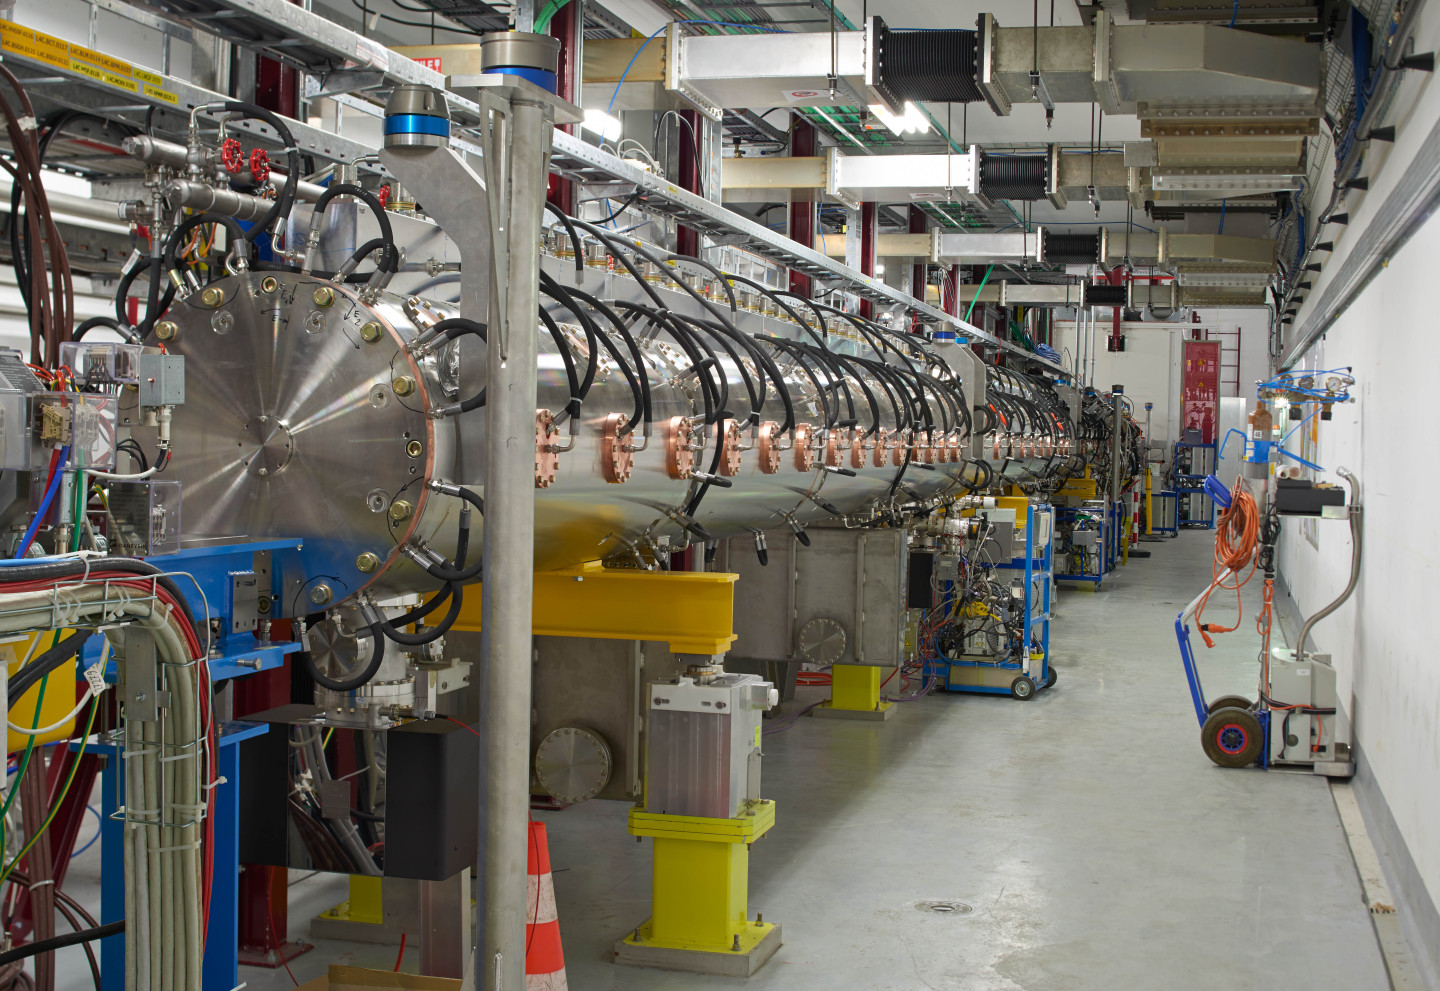
\includegraphics[width=\marginparwidth]{LHC/linac4.jpg}
 	\captionof{figure}{Photo du LINAC4.}
 	\label{linac4}
 }
 
 \item De nouvelles lignes de transmission électrique vont également être installées. Ces câbles seront faits d'un matériau supraconducteur \chemform{MgB_2} (diborure de magnésium), capable de fonctionner à haute température (\SI{20}{\kelvin}), beaucoup plus stables que les supraconducteurs conventionnels. Ils permettront de transporter des courants de plus de \SI{100}{\kilo\ampere}.
 \item La chaine d'accélération sera elle aussi mise à niveau. Dès \num{2020}, un nouvel accélérateur linéaire appelé LINAC4 (cf.Fig~\ref{linac4}) va remplacer le LINAC2. Les trois autres accélérateurs de la chaine (PSB, PS et SPS) auront également droit à des améliorations.
\end{itemize}

\begin{figure}[ht!]
	\centering
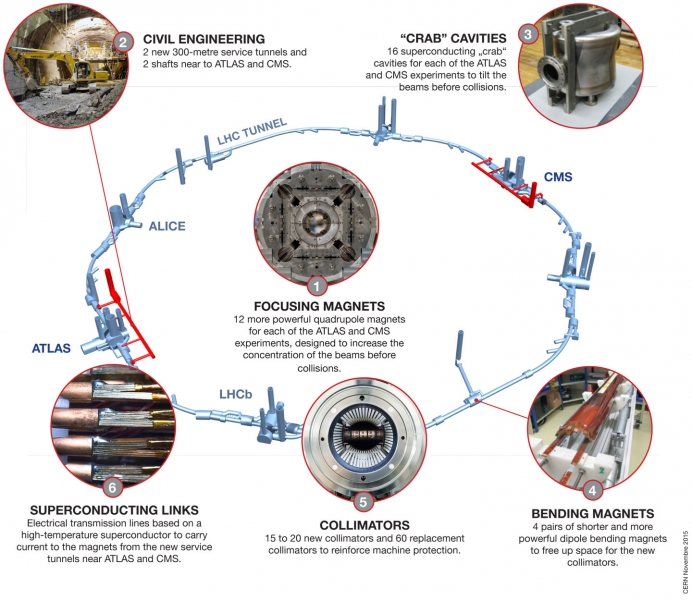
\includegraphics[width=0.58\textwidth]{LHC/man.jpg}
\captionof{figure}{Schéma montrant les différents types de mise à niveau nécessaires au HL-LHC \cite{High-Luminosity:2114692}.}
\label{man}	
\end{figure}

Le tableau \ref{comparaison} donne les différents paramètres selon plusieurs configurations envisagées par rapport aux paramètres nominaux actuels du LHC.

\begin{table}[!ht]
\tiny
\centering
\begin{tabular}{|O|Cc|Cc|Cc|Cc|N}
	\hline 
	\shortstack{Paramètre} &\shortstack{LHC Nominal\\(design report)}&\shortstack{HL-LHC \SI{25}{\nano\second}\\(standard)}&\shortstack{HL-LHC \SI{25}{\nano\second}\\(BCMS)}&\shortstack{HL-LHC\\8b+4e$^{12}$}\\ 
	\hline 
	\shortstack{Énergie du faisceau [\si{\tera\eV}]} & \shortstack{7} & \shortstack{7} & \shortstack{7} & \shortstack{7} \\ 
	\hline 
	\shortstack{Nombre de proton par paquet $N_{b}$}&\shortstack{\num{1.15e11}}&\shortstack{\num{2.2e11}}& \shortstack{\num{2.2e11}}&\shortstack{\num{2.3e11}}\\ 
	\hline 
	Nombres de paquets $n_{b}$& \num{2808} & \num{2748} & \num{2604} & \num{1968} \\ 
	\hline 
	\shortstack{Nombre de collisons aux point P1 et P5}& \num{2808} & \num{2736} & \num{2592} & \num{1960} \\ 
	\hline 
	Courant du faisceau [\si{\ampere}]& \num{0.58} & \num{1.09} & \num{1.03} & \num{0.82} \\ 
	\hline 
	angle x-ing [\si{\micro\radian}] & \num{285} & \num{590} & \num{590} & \num{554} \\ 
	\hline 
	$\beta{*}$ [\si{\meter}]& \num{0.55}  & \num{0.15} & \num{0.15} & \num{0.15} \\ 
	\hline 
	$\epsilon_{n}$ [\si{\micro\meter}]& \num{3.75} & \num{2.50} & \num{2.50} & \num{2.20} \\ 
	\hline 
	r.m.s. de la longueur du paquet [\si{\meter}]& \num{7.55e-2}  & \num{7.55e-2} & \num{7.55e-2} & \num{7.55e-2} \\ 
	\hline 
	paramètre de Piwinski & \num{0.65} & \num{3.14} & \num{3.14} & \num{3.14} \\ 
	\hline 
	\shortstack{Facteur de perte total $R0$ sans cavité "crabes"}& \num{0.836} & \num{0.305} & \num{0.305} & \num{0.304} \\ 
	\hline 
	\shortstack{Facteur de perte total $R1$ avec cavité "crabes"}& (\num{0.981}) & \num{0.829} & \num{0.829} & \num{0.828} \\ 
	\hline 
	\shortstack{Pic de luminosité sans cavité de type "crabe" [\si{\per\square\centi\meter\per\second}]}& \num{1.00e34} & \num{7.18e34} &\num{6.80e34} & \num{6.38e34} \\ 
	\hline 
	\shortstack{Luminosité virtuelle avec cavité de type "crabe" \\$L_{peak}R_{1}/R_{0}$[\si{\per\square\centi\meter\per\second}] } & \num{1.18e34} & \num{19.54e34} & \num{18.52e34} & \num{17.40e34} \\ 
	\hline 
	\shortstack{ Événements / croisement de faisceaux sans nivellement \\et sans cavités de type "crabe"}& \num{27} & \num{198} & \num{198} & \num{246} \\ 
	\hline 
	Luminosité nivellé [\si{\per\square\centi\meter\per\second}]& - & \num{5.00e34} &  \num{5.00e34}& \num{3.63e34} \\ 
	\hline 
	\shortstack{Événements/croisement de faisceaux avec nivellement \\ et cavités de type "crabe" pour HL-LHC}& \num{27} & \num{138} & \num{146} & \num{140} \\ 
	\hline 
	\shortstack{Pic de densité linéaire d'événement pile-up [evt/\si{\milli\meter}] \\(maximum pour des faisceaux stables)%Pic de densité linéaire d'événement pile-up \\ [événements/mm] (maximum pour des faisceaux stables)
	} & \shortstack{\num{0.21}} & \shortstack{\num{1.25}} & \shortstack{\num{1.31}} & \shortstack{\num{1.28}} \\ 
	\hline 
	\shortstack{temps de nivellement [\si{\hour}]\\ (aucune augmentation d'émittance)}& - & \num{8.3} & \num{7.6} & \num{9.5} \\ 
	\hline 
	$N_{b}$ à l'injection dans le LHC& \num{1.20e11} & \num{2.30e11} & \num{2.30e11} &\num{2.40e11}  \\ 
	\hline 
	$n_{b}$ par injection& \num{288} & \num{288} & \num{288} & \num{224} \\ 
	\hline 
	$\epsilon_{n}$ à l'extraction du SPS& \num{3.40} & \num{2.0} & $<$\num{2.00} & \num{1.70} \\ 
	\hline 
\end{tabular} 
\caption{Liste des principaux paramètres du faisceau du HL-LHC. La colonne intitulée "standard" est le design pris comme objectif, les deux autres colonnes représentent des variantes de ce design. Pour comparaison, les paramètres du faisceau du LHC dans son design nominal sont reportés dans la première colonne \cite{Apollinari:2116337}.}
\label{comparaison}
\end{table}

L'augmentation de la luminosité va aussi nécessiter la mise à niveau des détecteurs et notamment de CMS, afin de supporter le nombre important de collisions par croisement de faisceaux. D'autres améliorations et travaux de maintenance seront également réalisés durant cet arrêt. 